% ---------------------------------------------------------------
% TEMPLATE TCC1 - SENAC SANTO AMARO
% ---------------------------------------------------------------
% Trabalho de Conclusão de Curso 1
% Elaborado para apresentação da proposta inicial do TCC
% Estrutura: 4 capítulos (Introdução, Revisão Bibliográfica,
%            Desenvolvimento, Referências Bibliográficas)
% ---------------------------------------------------------------

\documentclass[
    12pt,                % tamanho da fonte
    openright,           % capítulos começam em página ímpar
    oneside,             % para impressão em apenas um lado do papel
    a4paper,             % tamanho do papel
    english,             % idioma adicional
    brazil               % idioma principal
]{abntex2}

% ---------------------------------------------------------------
% PACOTES
% ---------------------------------------------------------------
\usepackage{lmodern}                % Fonte Latin Modern
\usepackage[T1]{fontenc}            % Seleção de códigos de fonte
\usepackage[utf8]{inputenc}         % Codificação do documento
\usepackage{lastpage}               % Usado pela Ficha catalográfica
\usepackage{indentfirst}            % Indenta o primeiro parágrafo
\usepackage{color}                  % Controle de cores
\usepackage{graphicx}               % Inclusão de gráficos
\usepackage{microtype}              % Melhorias de justificação
\graphicspath{{assets/}{figuras/}}   % Diretórios de figuras
\usepackage{float}                  % Para posicionamento de figuras
\usepackage{tabularx}  
\usepackage{booktabs}               % Tabelas profissionais
\usepackage{multirow}               % Células mescladas em tabelas
\usepackage{longtable}              % Tabelas longas
\usepackage{amsmath,amssymb}        % Símbolos matemáticos
\usepackage{pgfgantt}               % Diagramas de Gantt
\usepackage[brazilian,hyperpageref]{backref}  % Páginas com citações
\usepackage[alf]{abntex2cite}       % Citações ABNT

% ---------------------------------------------------------------
% CONFIGURAÇÕES DO PDF
% ---------------------------------------------------------------
\makeatletter
\hypersetup{
    pdftitle={\@title},
    pdfauthor={\@author},
    pdfsubject={TCC1 - SENAC Santo Amaro},
    pdfcreator={LaTeX with abnTeX2},
    pdfkeywords={tcc}{senac}{santo amaro}{trabalho de conclusão},
    colorlinks=true,        % false: links em caixas; true: links coloridos
    linkcolor=blue,         % cor dos links internos
    citecolor=blue,         % cor dos links para bibliografia
    filecolor=magenta,      % cor dos links para arquivos
    urlcolor=blue,
    bookmarksdepth=4
}
\makeatother

% ---------------------------------------------------------------
% CONFIGURAÇÕES DE APARÊNCIA DO PDF FINAL
% ---------------------------------------------------------------
\definecolor{blue}{RGB}{41,5,195}

% ---------------------------------------------------------------
% INFORMAÇÕES DO DOCUMENTO
% ---------------------------------------------------------------
\titulo{Detecção de Fala Direcionada ao Computador Pessoal em Português Brasileiro: Uma Abordagem Textual para Assistentes de Voz sem Palavra de Ativação}
\autor{Phelipe Pereira de Souza}
\local{São Paulo}
\data{2026}
\orientador{Prof. Thyago Conchado Quintas}
% \coorientador{Prof. Nome do Coorientador} % Descomente se houver coorientador

\instituicao{%
  SENAC -- Serviço Nacional de Aprendizagem Comercial
  \par
  Unidade Santo Amaro
  \par
  Bacharelado em Ciência da Computação
}

\tipotrabalho{Trabalho de Conclusão de Curso I}

\preambulo{Proposta de Trabalho de Conclusão de Curso apresentado ao SENAC Santo Amaro como requisito parcial para aprovação na disciplina de TCC2 do Bacharelado em Ciência da Computação.}

% ---------------------------------------------------------------
% COMPILA O ÍNDICE
% ---------------------------------------------------------------
\makeindex

% ---------------------------------------------------------------
% INÍCIO DO DOCUMENTO
% ---------------------------------------------------------------
\begin{document}

% Seleciona o idioma do documento
\selectlanguage{brazil}

% Retira espaço extra obsoleto entre as frases
\frenchspacing

% ---------------------------------------------------------------
% ELEMENTOS PRÉ-TEXTUAIS
% ---------------------------------------------------------------
\pretextual

% ---------------------------------------------------------------
% CAPA
% ---------------------------------------------------------------
\imprimircapa

% ---------------------------------------------------------------
% FOLHA DE ROSTO
% ---------------------------------------------------------------
\imprimirfolhaderosto

% ---------------------------------------------------------------
% RESUMO
% ---------------------------------------------------------------
% \begin{resumo}

    
% \vspace{\onelineskip}

% \noindent
% % \textbf{Palavras-chave}: palavra1. palavra2. palavra3. palavra4. palavra5.
% \end{resumo}

% ---------------------------------------------------------------
% LISTA DE ILUSTRAÇÕES
% ---------------------------------------------------------------
\pdfbookmark[0]{\listfigurename}{lof}
\listoffigures*
\cleardoublepage

% ---------------------------------------------------------------
% LISTA DE TABELAS
% ---------------------------------------------------------------
\pdfbookmark[0]{\listtablename}{lot}
\listoftables*
\cleardoublepage

% ---------------------------------------------------------------
% LISTA DE ABREVIATURAS E SIGLAS
% ---------------------------------------------------------------
\begin{siglas}
  \item[ASR] \textit{Automatic Speech Recognition} (Reconhecimento Automático de Fala)
  \item[DDSD] \textit{Device-Directed Speech Detection} (Detecção de Fala Direcionada ao Dispositivo)
  \item[EER] \textit{Equal Error Rate} (Taxa de Erro Igual)
  \item[HCI] \textit{Human-Computer Interaction} (Interação Humano-Computador)
  \item[HMM] \textit{Hidden Markov Model} (Modelo Oculto de Markov)
  \item[LLM] \textit{Large Language Model} (Modelo de Linguagem de Grande Porte)
  \item[LR] \textit{Logistic Regression} (Regressão Logística)
  \item[ML] \textit{Machine Learning} (Aprendizado de Máquina)
  \item[NLP] \textit{Natural Language Processing} (Processamento de Linguagem Natural)
  \item[NLU] \textit{Natural Language Understanding} (Compreensão de Linguagem Natural)
  \item[SVM] \textit{Support Vector Machines} (Máquinas de Vetores de Suporte)
  \item[TF-IDF] \textit{Term Frequency-Inverse Document Frequency} (Frequência do Termo - Inverso da Frequência nos Documentos)
  \item[TTS] \textit{Text-to-Speech} (Síntese de Fala)
  \item[VAD] \textit{Voice Activity Detection} (Detecção de Atividade de Voz)
  \item[WER] \textit{Word Error Rate} (Taxa de Erro de Palavras)
\end{siglas}
\cleardoublepage

% ---------------------------------------------------------------
% SUMÁRIO
% ---------------------------------------------------------------
\pdfbookmark[0]{\contentsname}{toc}
\tableofcontents*
\cleardoublepage

% ---------------------------------------------------------------
% ELEMENTOS TEXTUAIS
% ---------------------------------------------------------------
\textual

% ===============================================================
% CAPÍTULO 1 - INTRODUÇÃO
% ===============================================================
\chapter{Introdução}
\label{cap:introducao}

Nas últimas décadas, os assistentes de voz tornaram-se componentes cada vez mais presentes no cotidiano, incorporados a \textit{smartphones}, alto-falantes inteligentes, \textit{wearables}, computadores pessoais e sistemas de automação residencial~\cite{Jurafsky2024}. Esses sistemas permitem que usuários interajam com dispositivos computacionais por meio de comandos de voz, facilitando a execução de tarefas como busca de informações, abertura de aplicativos e gerenciamento de atividades. O mercado global de assistentes de voz foi avaliado em US\$ 7,35 bilhões em 2024 e projeta-se que alcance US\$ 33,74 bilhões até 2030, com taxa de crescimento anual composta de 26,5\%, o que evidencia a escala e a relevância dessa tecnologia, conforme ilustrado no gráfico de projeção da Figura~\ref{fig:market}~\cite{NMSC2025}.

\begin{figure}[htb]       
    \centering           
    \caption{Projeção de crescimento do mercado global de assistentes virtuais de voz (2024--2030).}
    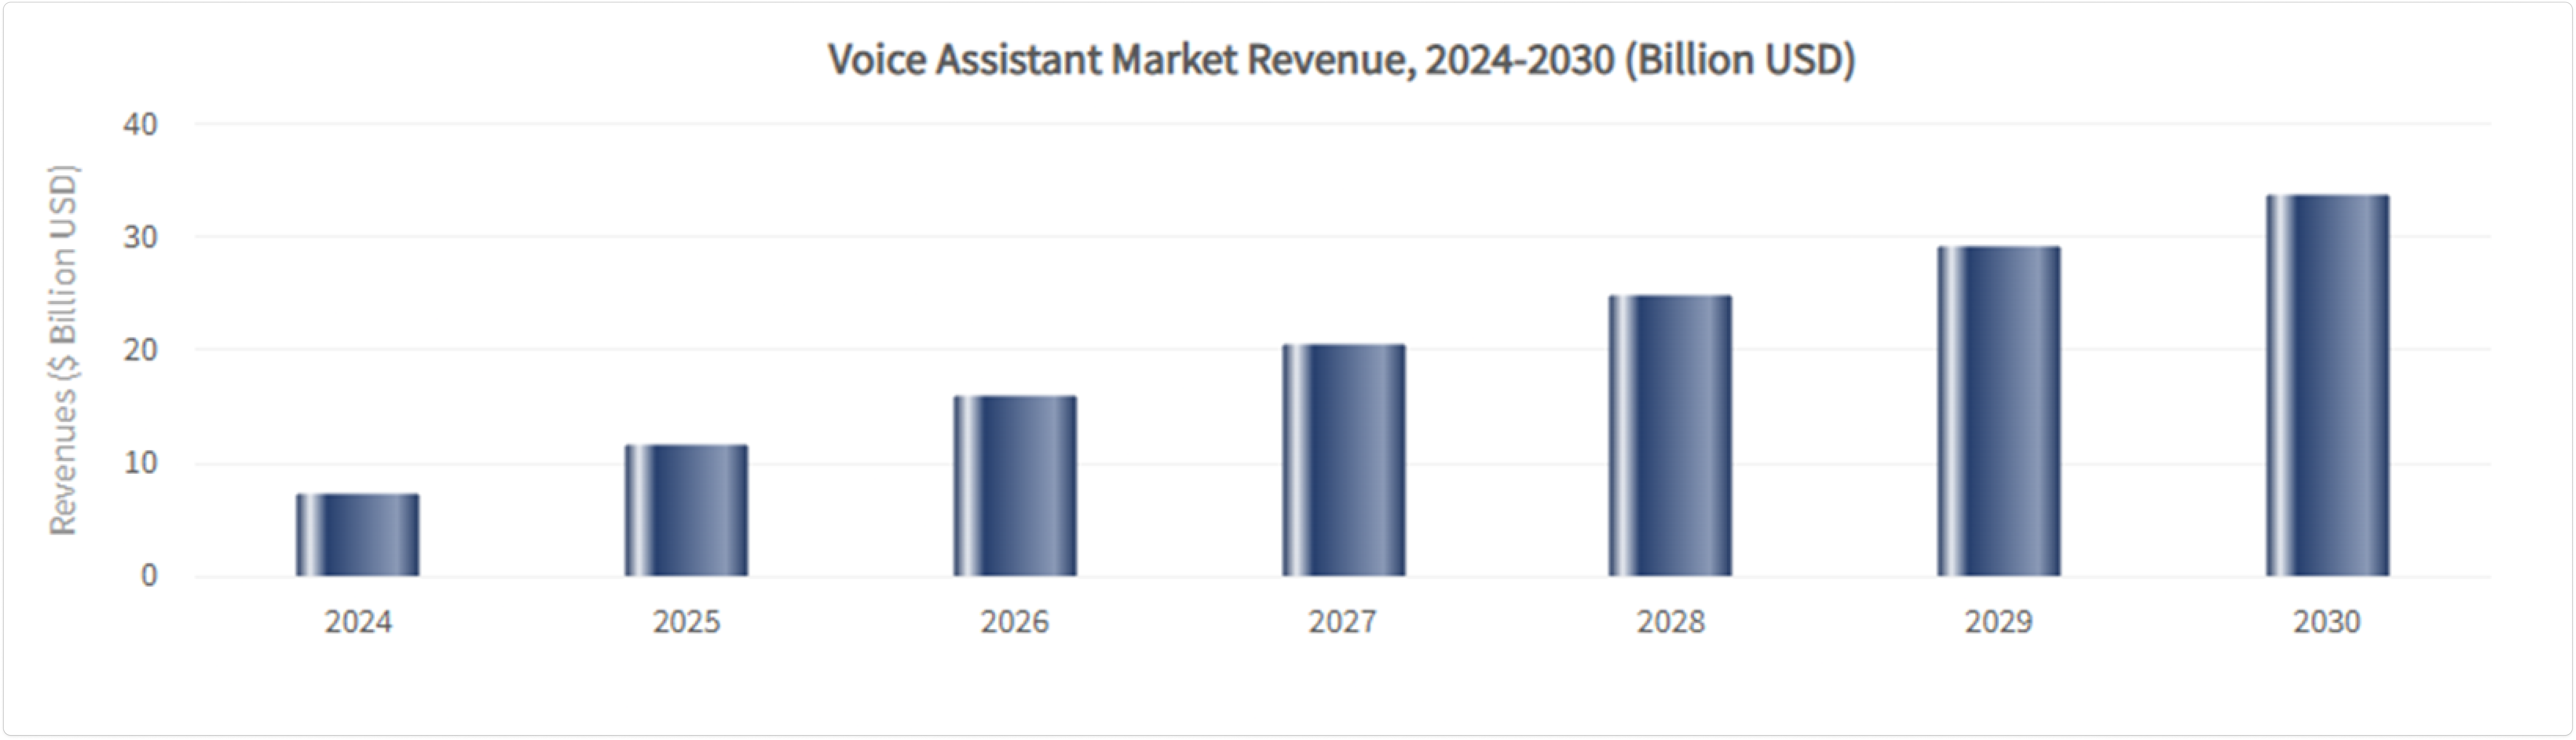
\includegraphics[width=1.0\textwidth]{market.png} 
    \fonte{Next Move Strategy Consulting (2025).}
    \label{fig:market}
\end{figure}

Na maioria dos sistemas atuais, a interação com assistentes de voz é iniciada por meio de palavras de ativação explícitas, conhecidas como \textit{wake-words} ou \textit{hotwords}, tais como ``Hey Siri'', ``Alexa'' ou ``Ok Google''. Essas expressões atuam como um mecanismo de gatilho que sinaliza ao sistema o desejo do usuário de iniciar uma interação. Do ponto de vista técnico, essa abordagem é eficaz, pois permite reduzir o processamento contínuo de áudio e minimizar ativações indevidas \cite{Garg2021}. No entanto, a dependência de \textit{wake-words} impõe limitações significativas à naturalidade da comunicação humano-computador, tornando a interação menos fluida e intuitiva quando comparada ao diálogo humano \cite{Nie2021}.

Em interações humanas cotidianas, comandos e solicitações são frequentemente expressos de forma implícita, inseridos naturalmente no fluxo da conversação, sem a necessidade de uma palavra específica para iniciar a comunicação \cite{Weld2022}. Os sistemas baseados em \textit{wake-words}, por sua vez, exigem que o usuário diga uma palavra específica para iniciar a interação, o que torna a comunicação menos natural. Além disso, esses sistemas são vulneráveis ao fenômeno de ativações falsas provocadas por palavras foneticamente semelhantes, conhecido como \textit{FakeWake} \cite{Chen2021}. Esses problemas comprometem a experiência do usuário e evidenciam as limitações dessa abordagem para tornar a interação mais natural e intuitiva.

Nesse cenário, surge a área de pesquisa denominada \textit{Device-Directed Speech Detection} (traduzido como Detecção de Fala Direcionada ao Dispositivo, referenciado pela sigla DDSD), que visa determinar automaticamente se uma fala é direcionada a um assistente virtual, mesmo na ausência de uma palavra de ativação explícita, ou se faz parte de uma conversa entre humanos \cite{Mallidi2018, Wagner2024}. Essa abordagem possibilita interações mais naturais e fluidas, reduzindo a necessidade de gatilhos verbais explícitos (\textit{wake-words}) e representando um avanço significativo rumo a uma comunicação humano-computador mais intuitiva e semelhante ao diálogo cotidiano.

Entre os diferentes usos do assistente de voz, o computador pessoal merece destaque por fazer parte de muitas atividades do dia a dia, como estudar, trabalhar e se divertir. Nesses dispositivos, o usuário pode abrir programas, fazer pesquisas na \textit{web}, reproduzir conteúdos e realizar outras tarefas por meio de comandos de voz, sem precisar usar o teclado ou o \textit{mouse}. No entanto, esse tipo de uso traz um desafio específico para a DDSD: computadores costumam ser utilizados em ambientes compartilhados, como escritórios, laboratórios e residências. Nesses locais, é comum que o usuário converse com outras pessoas, enquanto utiliza o computador. Durante essas conversas, nomes de aplicativos e \textit{sites} populares podem ser mencionados sem que haja qualquer intenção de interagir com o assistente de voz.

Este trabalho investiga a viabilidade da DDSD em português brasileiro, no contexto de assistentes de voz para computadores pessoais, por meio de uma abordagem baseada exclusivamente no nível textual. O sistema opera com transcrições de fala obtidas via Reconhecimento Automático de Fala (do inglês \textit{Automatic Speech Recognition}, referido pela sigla ASR), e aplica técnicas de Processamento de Linguagem Natural (do inglês \textit{Natural Language Processing}, referido pela sigla NLP) e Aprendizado de Máquina (do inglês \textit{Machine Learning}, referido pela sigla ML) para classificar automaticamente se uma fala é um comando direcionado ao computador ou faz parte de uma conversa incidental entre humanos. O foco deste trabalho reside na etapa de decisão de direcionamento, tratando o ASR como um módulo de pré-processamento encarregado de gerar as transcrições textuais que servirão de entrada para o classificador. A interpretação do comando e a execução da ação correspondente não fazem parte do escopo.

% ---------------------------------------------------------------

\section{Cenário motivador}
\label{sec:cenario}

Para entender melhor o problema e sua importância, considere o cenário apresentado na Figura~\ref{fig:cenario}. Um usuário está em frente ao computador, com o assistente de voz ativo e o microfone captando continuamente os sons do ambiente. Um colega se aproxima e os dois começam a conversar. Durante a conversa, o usuário pergunta: ``você viu aquele vídeo novo no YouTube?'' (Cenário A). Mesmo que o microfone capte a fala e que ela mencione um serviço acessível pelo assistente, nenhuma ação deve ser executada, pois a pergunta é dirigida ao colega, e não ao computador. Em outro momento, o usuário volta a atenção para o monitor e diz: ``abre o YouTube e pesquisa receitas de bolo'' (Cenário B). Nesse caso, o assistente deve identificar que o comando é direcionado a ele e executar a tarefa solicitada, mesmo sem o uso de uma \textit{wake-word}.

\begin{figure}[htb]       
    \centering           
    \caption{Cenário ilustrativo de Detecção de Fala Direcionada ao Dispositivo (DDSD) em um computador pessoal.}
    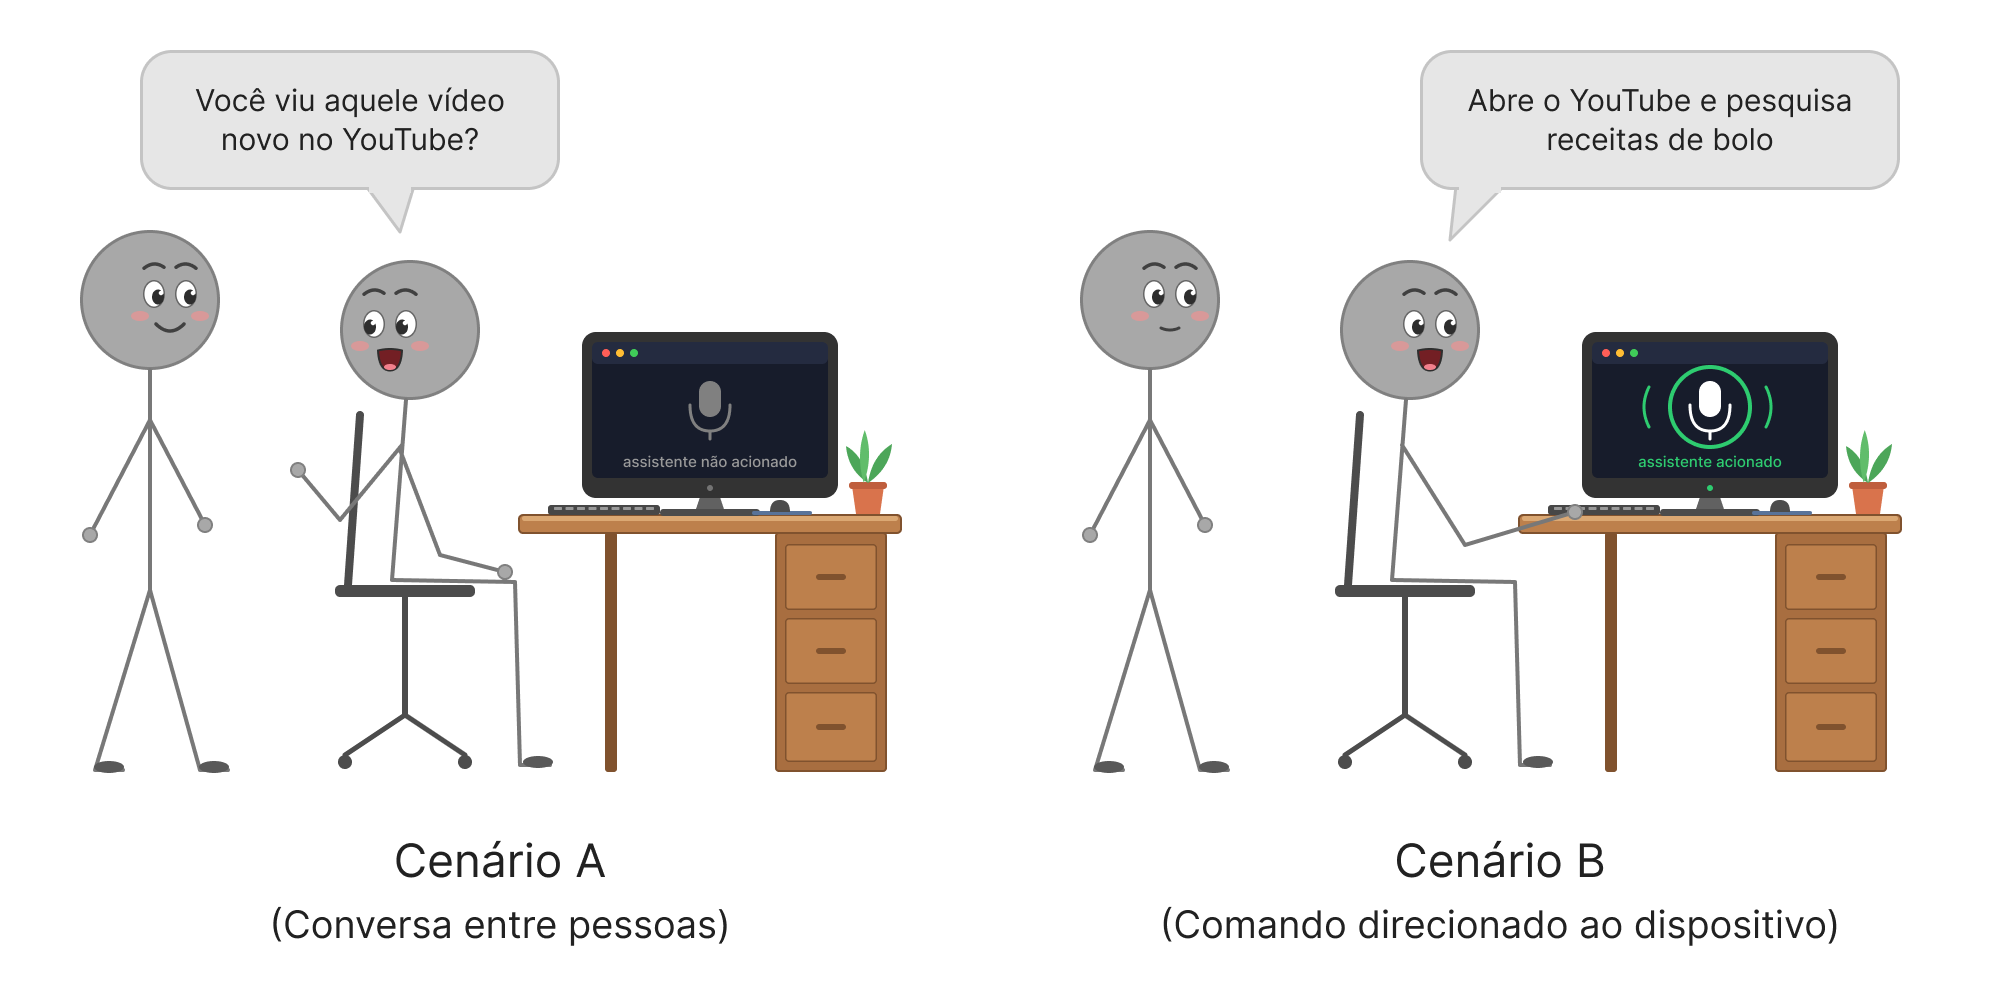
\includegraphics[width=0.75\textwidth]{cenario.png} 
    \fonte{Elaborado pelo autor (2026).}
    \label{fig:cenario}
\end{figure}

A comparação entre os dois enunciados mostra que a presença de palavras-chave, como o nome de um aplicativo ou site, não é suficiente para determinar se uma fala é direcionada ao assistente. É necessário considerar o conteúdo do enunciado e a inteção por trás dele. Nesse contexto, o sistema precisa distinguir duas categorias de fala: (i) comandos direcionados ao dispositivo (DD, do inglês \textit{Device-Directed}), como ``abre o YouTube e pesquisa receitas de bolo''; e (ii) comentários e conversas que não são direcionadas ao dispositivo (NDD, do inglês \textit{Non-Device-Directed}), como ``você viu aquele vídeo novo no YouTube?''. A DDSD tem como objetivo realizar essa distinção automaticamente, sem depender de \textit{wake-words} explícitas \cite{Mallidi2018, Wagner2024}. Neste trabalho, essa classificação é feita apenas com base no conteúdo textual do enunciado transcrito, sem utilizar informações visuais, como a direção do olhar, ou acústicas, como a entoação da voz.

% ---------------------------------------------------------------
\section{Contexto}
\label{sec:contexto}

Os avanços em ASR e NLP têm contribuído para o desenvolvimento de assistentes de voz mais eficientes. Entre os modelos disponíveis, o Whisper \cite{Radford2023} se destaca pela capacidade de transcrever áudios com boa precisão em diferentes idiomas. A \citeonline{OpenAI2024Turbo} lançou o Whisper Large V3 Turbo, uma versão otimizada que reduz o número de camadas do decodificador de 32 para 4, tornando a transcrição mais rápida e mantendo um desempenho próximo ao do modelo original. Neste trabalho, essa versão é utilizada como módulo principal de ASR por combinar precisão e velocidade, permitindo sua execução local em um computador pessoal sem exigir tantos recursos computacionais quanto o modelo completo. Outras alternativas também foram propostas na literatura, como o Whispy \cite{Bevilacqua2024}, que adapta o Whisper para o processamento contínuo de áudio (\textit{streaming}), e o Moonshine \cite{Jeffries2024}, um modelo mais compacto desenvolvido para funcionar em dispositivos com recursos computacionais limitados.

A arquitetura Transformer \cite{Vaswani2017} também teve um papel importante no avanço do NLP e serviu de base para o desenvolvimento dos atuais modelos de linguagem de grande porte (LLMs, do inglês \textit{Large Language Models}). Para o português brasileiro, o BERTimbau \cite{Souza2020} se tornou uma alternativa importante para tarefas de compreensão de texto e é utilizado neste trabalho como classificador principal de direcionamento. Outros modelos também ampliaram as opções disponíveis para o idioma, como o Albertina \cite{Rodrigues2023} e o DeBERTinha \cite{Abonizio2023}, sendo este último desenvolvido a partir do DeBERTaV3 XSmall, com foco em reduzir a quantidade de parâmetros. Além disso, a disponibilidade de LLMs generativos capazes de trabalhar com diferentes idiomas permite gerar grandes volumes de textos sintéticos em português. Neste trabalho, esse recurso é utilizado para construir o corpus de dados.

Para esclarecer a função de cada família de modelos neste projeto, a Tabela~\ref{tab:tecnologias} apresenta como as responsabilidades são distribuídas entre elas.

\begin{table}[H]
\caption{Tecnologias utilizadas e seus papéis no trabalho}
\label{tab:tecnologias}
\begin{tabular}{lll}
\toprule
\textbf{Tecnologia} & \textbf{Papel no trabalho} & \textbf{Implementada?} \\
\midrule
Whisper Large V3 Turbo & ASR: transcrição de áudio & Sim (principal) \\
Moonshine/Whispy & ASR: alternativa discutida na literatura & Não \\
BERTimbau & Classificação de direcionamento (DDSD) & Sim (principal) \\
DeBERTinha & Classificação de direcionamento (DDSD) & Sim (alternativo) \\
Albertina & Classificação de direcionamento (DDSD) & Sim (alternativo) \\
TF-IDF + SVM/LR & Classificação: baseline clássico & Sim \\
LLMs generativos & Geração de dados sintéticos & Sim \\
\bottomrule
\end{tabular}
\fonte{Elaborado pelo autor (2026).}
\end{table}

Pesquisas recentes sobre DDSD têm explorado o uso do texto como alternativa para reduzir as limitações de abordagens baseadas apenas em características acústicas. Estudos como os de \citeonline{Wagner2024, Dighe2024} mostram que classificadores baseados em Transformers podem analisar transcrições geradas por sistemas de ASR para identificar se um enunciado é direcionado ao dispositivo. De forma semelhante, \citeonline{Rudovic2024} investigaram como o significado das palavras pode ajudar a identificar intenções implícitas em diálogos contínuos. Esses trabalhos reforçam a possibilidade de utilizar apenas o conteúdo textual das transcrições para realizar a classificação de direcionamento.

% ---------------------------------------------------------------
\section{Justificativa}
\label{sec:justificativa}

O uso cada vez mais comum de assistentes de voz em diferentes dispositivos reforça a importância de pesquisas voltadas à melhoria da Interação Humano-Computador (HCI, do inglês \textit{Human-Computer Interaction}). Embora tenham ocorrido avanços em ASR e NLP, muitos sistemas ainda exigem o uso de palavras de ativação para iniciar uma interação, o que pode tornar a comunicação menos natural \cite{Mallidi2018}. Quando um usuário precisa interagir com o dispositivo várias vezes ao longo do dia, a repetição desse processo pode causar cansaço e prejudicar a experiência de uso \cite{Nie2021}. Nesse contexto, a DDSD surge como uma alternativa para reduzir a dependência dessas palavras de ativação e tornar a interação com assistentes de voz mais simples e fluida \cite{Wagner2024}.

No caso dos computadores pessoais, dispensar o uso de uma \textit{wake-word} pode trazer benefícios importantes. Como o computador costuma ser utilizado por longos períodos, o usuário pode precisar dar vários comandos de voz durante uma mesma sessão, seja para abrir programas, alternar entre janelas ou realizar pesquisas. Nesse contexto, ter que repetir uma palavra de ativação a cada interação pode tornar o uso menos prático. A interação por voz sem esse requisito também pode facilitar o uso do computador por pessoas com limitações motoras que dificultam o uso do teclado e do \textit{mouse}, além de ser útil quando as mão estão ocupadas. No entanto, como os computadores também são utilizados em ambientes compartilhados, o microfone pode captar conversas que não são direcionadas ao assistente. Por isso, é importante que o sistema consiga diferenciar os comandos destinados ao computador das falas que fazem parte de conversas comuns.

Do ponto de vista acadêmico, o estudo de alternativas para ativar assistentes de voz com base no direcionamento da fala envolve três áreas: processamento de áudio, NLP e HCI. Embora estudos indiquem que a combinação de informações acústicas e textuais pode reduzir os erros de ativação \cite{Wagner2024}, essa abordagem também apresenta desafios. Sistemas multimodais exigem mais recursos computacionais, precisam sincronizar diferentes tipos de sinais e dependem de grandes volumes de dados rotulados, tanto de áudio quanto de texto. Esses requisitos podem dificultar sua implementação em dispositivos com recursos limitados \cite{Xu2024}. Em contrapartida, uma abordagem baseada apenas no texto transcrito exige menos recursos computacionais e pode ser executada no próprio computador do usuário, sem depender de serviços em nuvem.

Adicionalmente, identifica-se uma lacuna geográfica e linguística na literatura: os principais estudos sobre DDSD concentram-se quase exclusivamente no idioma inglês, com forte dependência de características acústicas e prosódicas nativas daquela língua \cite{Norouzian2019, Krishna2023}. O português brasileiro, apesar de ser um dos idiomas mais falados do mundo, apresenta-se sub-representado nesse campo de pesquisa, carecendo de estudos focados na decodificação de padrões de direcionamento de fala adaptados à sua realidade gramatical e cultural.

Embora o ecossistema nacional tenha presenciado o surgimento de recursos linguísticos robustos, como o BERTimbau \cite{Souza2020} e corpora públicos de fala (ex.: CORAA ASR \cite{CORAA2023}, NURC-SP \cite{NURCSP2025}, TAGARELA \cite{Tagarela2026}), tais bases destinam-se prioritariamente a tarefas de transcrição ortográficas e reconhecimento automático de fala. Verifica-se, portanto, uma escassez de corpora especificamente anotados com fins de detecção de direcionamento de voz (DD vs NDD) em português brasileiro, constituindo um gargalo para a pesquisa científica e o desenvolvimento de soluções práticas para DDSD nesse idioma.

Diante dessa lacuna, este trabalho investiga a viabilidade de uma abordagem de DDSD baseada apenas em texto, voltada à identificação de comandos de voz em computadores pessoais. Para isso, são utilizadas transcrições geradas por sistemas de ASR e modelos baseados em Transformer pré-treinados para o português brasileiro. A escolha por uma abordagem textual considera três aspectos principais: (i) a capacidade dos modelos baseados em atenção de identificar relações semânticas e intenções implícitas em enunciados curtos \cite{Weld2022}; (ii) as evidências de que o conteúdo linguístico das transcrições automáticas pode ajudar a distinguir comandos de conversas comuns \cite{Wagner2024, Dighe2024}; e (iii) a possibilidade de manter a classificação textual separada do módulo de transcrição, facilitando a comparação com métodos tradicionais de classificação e a análise dos efeitos de ruídos e erros de transcrição sobre os resultados \cite{Dighe2024}.

% ---------------------------------------------------------------

\section{Hipótese de pesquisa}
\label{sec:hipotese}

\textit{Sob condições de ambiente controlado e no domínio de comandos de voz para computadores pessoais, modelos de linguagem pré-treinados para o português brasileiro, aplicados sobre transcrições geradas por sistemas de ASR, alcançam desempenho estatisticamente superior a baselines lineares tradicionais, constituídos pela representação TF-IDF combinada com SVM ou LR, avaliados sobre o mesmo corpus sob as métricas de F1-score, acurácia e EER, evidenciando o ganho da abordagem baseada em Transformers para a tarefa de DDSD Textual em português brasileiro.}

Essa conjectura encontra sustentação nos fundamentos apresentados na Seção~\ref{sec:fundamentos}: a viabilidade da classificação puramente textual sobre as transcrições de ASR \cite{Wagner2024}, a superioridade de arquiteturas Transformer em tarefas de classificação de intenção \cite{Weld2022} e o desempenho comprovado de modelos especializados no português brasileiro, como o BERTimbau \cite{Souza2020} e o DeBERTinha \cite{Abonizio2023}. 

A validação dessa hipótese será realizada por meio de experimentos controlados, utilizando um corpus anotado especificamente para a tarefa de DDSD em português brasileiro, com comparação rigorosa entre o modelo baseado em Transformer e os \textit{baselines} lineares definidos nos Objetivos Específicos.

% ---------------------------------------------------------------
\section{Objetivos}
\label{sec:objetivos}

\subsection{Objetivo principal}

O objetivo principal desta pesquisa consiste em avaliar a viabilidade técnica e o desempenho de modelos de linguagem pré-treinados para o português brasileiro aplicados à DDSD no domínio de interação por voz com computadores pessoais, operando sobre transcrições puramente textuais geradas por sistemas de ASR, de modo a verificar se essa abordagem supera estatisticamente os \textit{baselines} lineares compostos por TF-IDF associado a SVM ou LR, nas métricas de F1-score, acurácia e EER.

\subsection{Objetivos específicos}

Para que o objetivo principal seja alcançado, foram definidos os seguintes objetivos específicos:

\begin{enumerate}
    \item Construir e validar um corpus balanceado de enunciados em português brasileiro no domínio de interação com o computador pessoal, anotados com base no direcionamento de fala (DD e NDD) sob critérios explícitos de anotação e de exclusão, a partir de enunciados sintéticos controlados gerados por LLMs de múltiplos provedores.

    \item Implementar, ajustar (\textit{fine-tuning}) e avaliar os modelos BERTimbau \cite{Souza2020}, DeBERTinha \cite{Abonizio2023} e Albertina \cite{Rodrigues2023} na tarefa de classificação binária de DDSD, confrontando empiricamente seus resultados com um \textit{baseline} composto pela representação vetorial TF-IDF aliada a SVM ou LR, utilizando transcrições geradas por ASR.

    \item Analisar o impacto gerado por erros e ruídos de transcrição automática no classificador de direcionamento, mapeando o desempenho comparativo entre o texto de referência e as transcrições automáticas e estabelecendo a correlação estatística entre a \textit{Word Error Rate} (traduzida como Taxa de Erro de Palavras, referenciada pela sigla WER) das saídas do ASR e o decaimento de desempenho do classificador textual \cite{Dighe2024}.

    \item Avaliar se os classificadores treinados conseguem generalizar para situações de fala real, utilizando transcrições de corpora públicos de português brasileiro, como CORAA \cite{CORAA2023}, NURC-SP \cite{NURCSP2025} e TAGARELA \cite{Tagarela2026}. Como esses corpora contêm conversas, entrevistas e diálogos entre pessoas, seus enunciados serão utilizados para avaliar a capacidade dos modelos de reconhecer falas não direcionadas ao dispositivo (NDD) e medir a taxa de falsas ativações.
\end{enumerate}

% ---------------------------------------------------------------

\section{Limitações do trabalho}
\label{sec:limitacoes}

Este trabalho apresenta algumas limitações relacionadas ao seu escopo e à metodologia adotada, que devem ser consideradas na análise dos resultados.

A primeira limitação está relacionada ao uso exclusivo de informações textuais. O classificador analisa apenas as transcrições dos enunciados, sem considerar características acústicas e prosódicas da fala, como entonação, velocidade e pausas, que também podem ajudar a identificar se uma fala é direcionada ao dispositivo \cite{Norouzian2019, Krishna2023}. Essa escolha permite avaliar a capacidade do texto de distinguir comandos de conversas comuns, mas também limita as informações disponíveis para a classificação. Por isso, o desempenho do sistema pode ser afetado por erros de transcrição e por situações em que as características da voz seriam úteis para identificar a intenção do falante.

A segunda limitação está relacionada aos erros de transcrição do ASR e às condições do áudio utilizado na avaliação. Como o classificador recebe o texto gerado pelo Whisper, erros de reconhecimento ou omissões podem alterar o significado dos enunciados e prejudicar a classificação feita pelo Transformer. Esse problema pode ser mais frequente em falas com sotaques, ruídos de fundo ou palavras pouco comuns \cite{Bevilacqua2024}

A terceira limitação diz respeito à construção do corpus experimental e à sua capacidade de representar a diversidade da fala real. Como há poucos conjuntos de dados específicos para DDSD em português brasileiro, este trabalho utiliza um corpus próprio, construído com o auxílio de LLMs para gerar enunciados sintéticos. Embora essa estratégia permita criar dados voltados ao problema estudado, ela apresenta limitações quanto à espontaneidade das conversas, à diversidade regional e sociolinguística e às variações de sotaque e de uso da língua. Dessa forma, o corpus não representa toda a variedade encontrada em situações reais de comunicação, o que pode limitar a generalização dos resultados \cite{CORAA2023}.

A quarta limitação está relacionada à classificação binária dos enunciados e à análise de cada fala de forma isolada. O sistema classifica cada enunciado sem considerar o histórico da conversa ou informações externas ao texto.

Por fim, este trabalho não avalia os aspectos necessários para a implantação do sistema em um ambiente de produção, como a latência de todo o processo, o armazenamento de áudio, a segurança dos dados e a privacidade dos usuários. A pesquisa se concentra na avaliação experimental e estatística da classificação textual em um ambiente controlado. Questões relacionadas à arquitetura do sistema, às exigências regulatórias, à proteção da privacidade e ao consentimento dos usuários ficam fora do escopo deste estudo e deverão ser consideradas em trabalhos futuros \cite{Chen2021}.

% ===============================================================
% CAPÍTULO 2 - REVISÃO BIBLIOGRÁFICA
% ===============================================================
\chapter{Revisão Bibliográfica}
\label{cap:revisao}

Este capítulo estabelece o embasamento teórico e tecnológico da pesquisa proposta. Inicialmente, descreve-se a metodologia de seleção dos trabalhos consultados. O referencial teórico, na sequência, percorre os paradigmas de interação por voz, desde os mecanismos tradicionais de ativação baseados em \textit{wake-words} até as abordagens emergentes de Detecção de Fala Direcionada ao Dispositivo (do inglês \textit{Device-Directed Speech Detection}, referida pela sigla DDSD). Os fundamentos técnicos são então aprofundados, com ênfase na arquitetura Transformer, nos modelos de linguagem pré-treinados para o português brasileiro e nas métricas de avaliação. Por fim, analisam-se os trabalhos mais diretamente relacionados ao tema, identificando lacunas que esta pesquisa busca preencher.

\section{Metodologia da pesquisa bibliográfica}
\label{sec:metodologia_pesquisa}

\begin{figure}[htb]       
    \centering           
    \caption{Fluxo de seleção de estudos para a revisão bibliográfica.}
    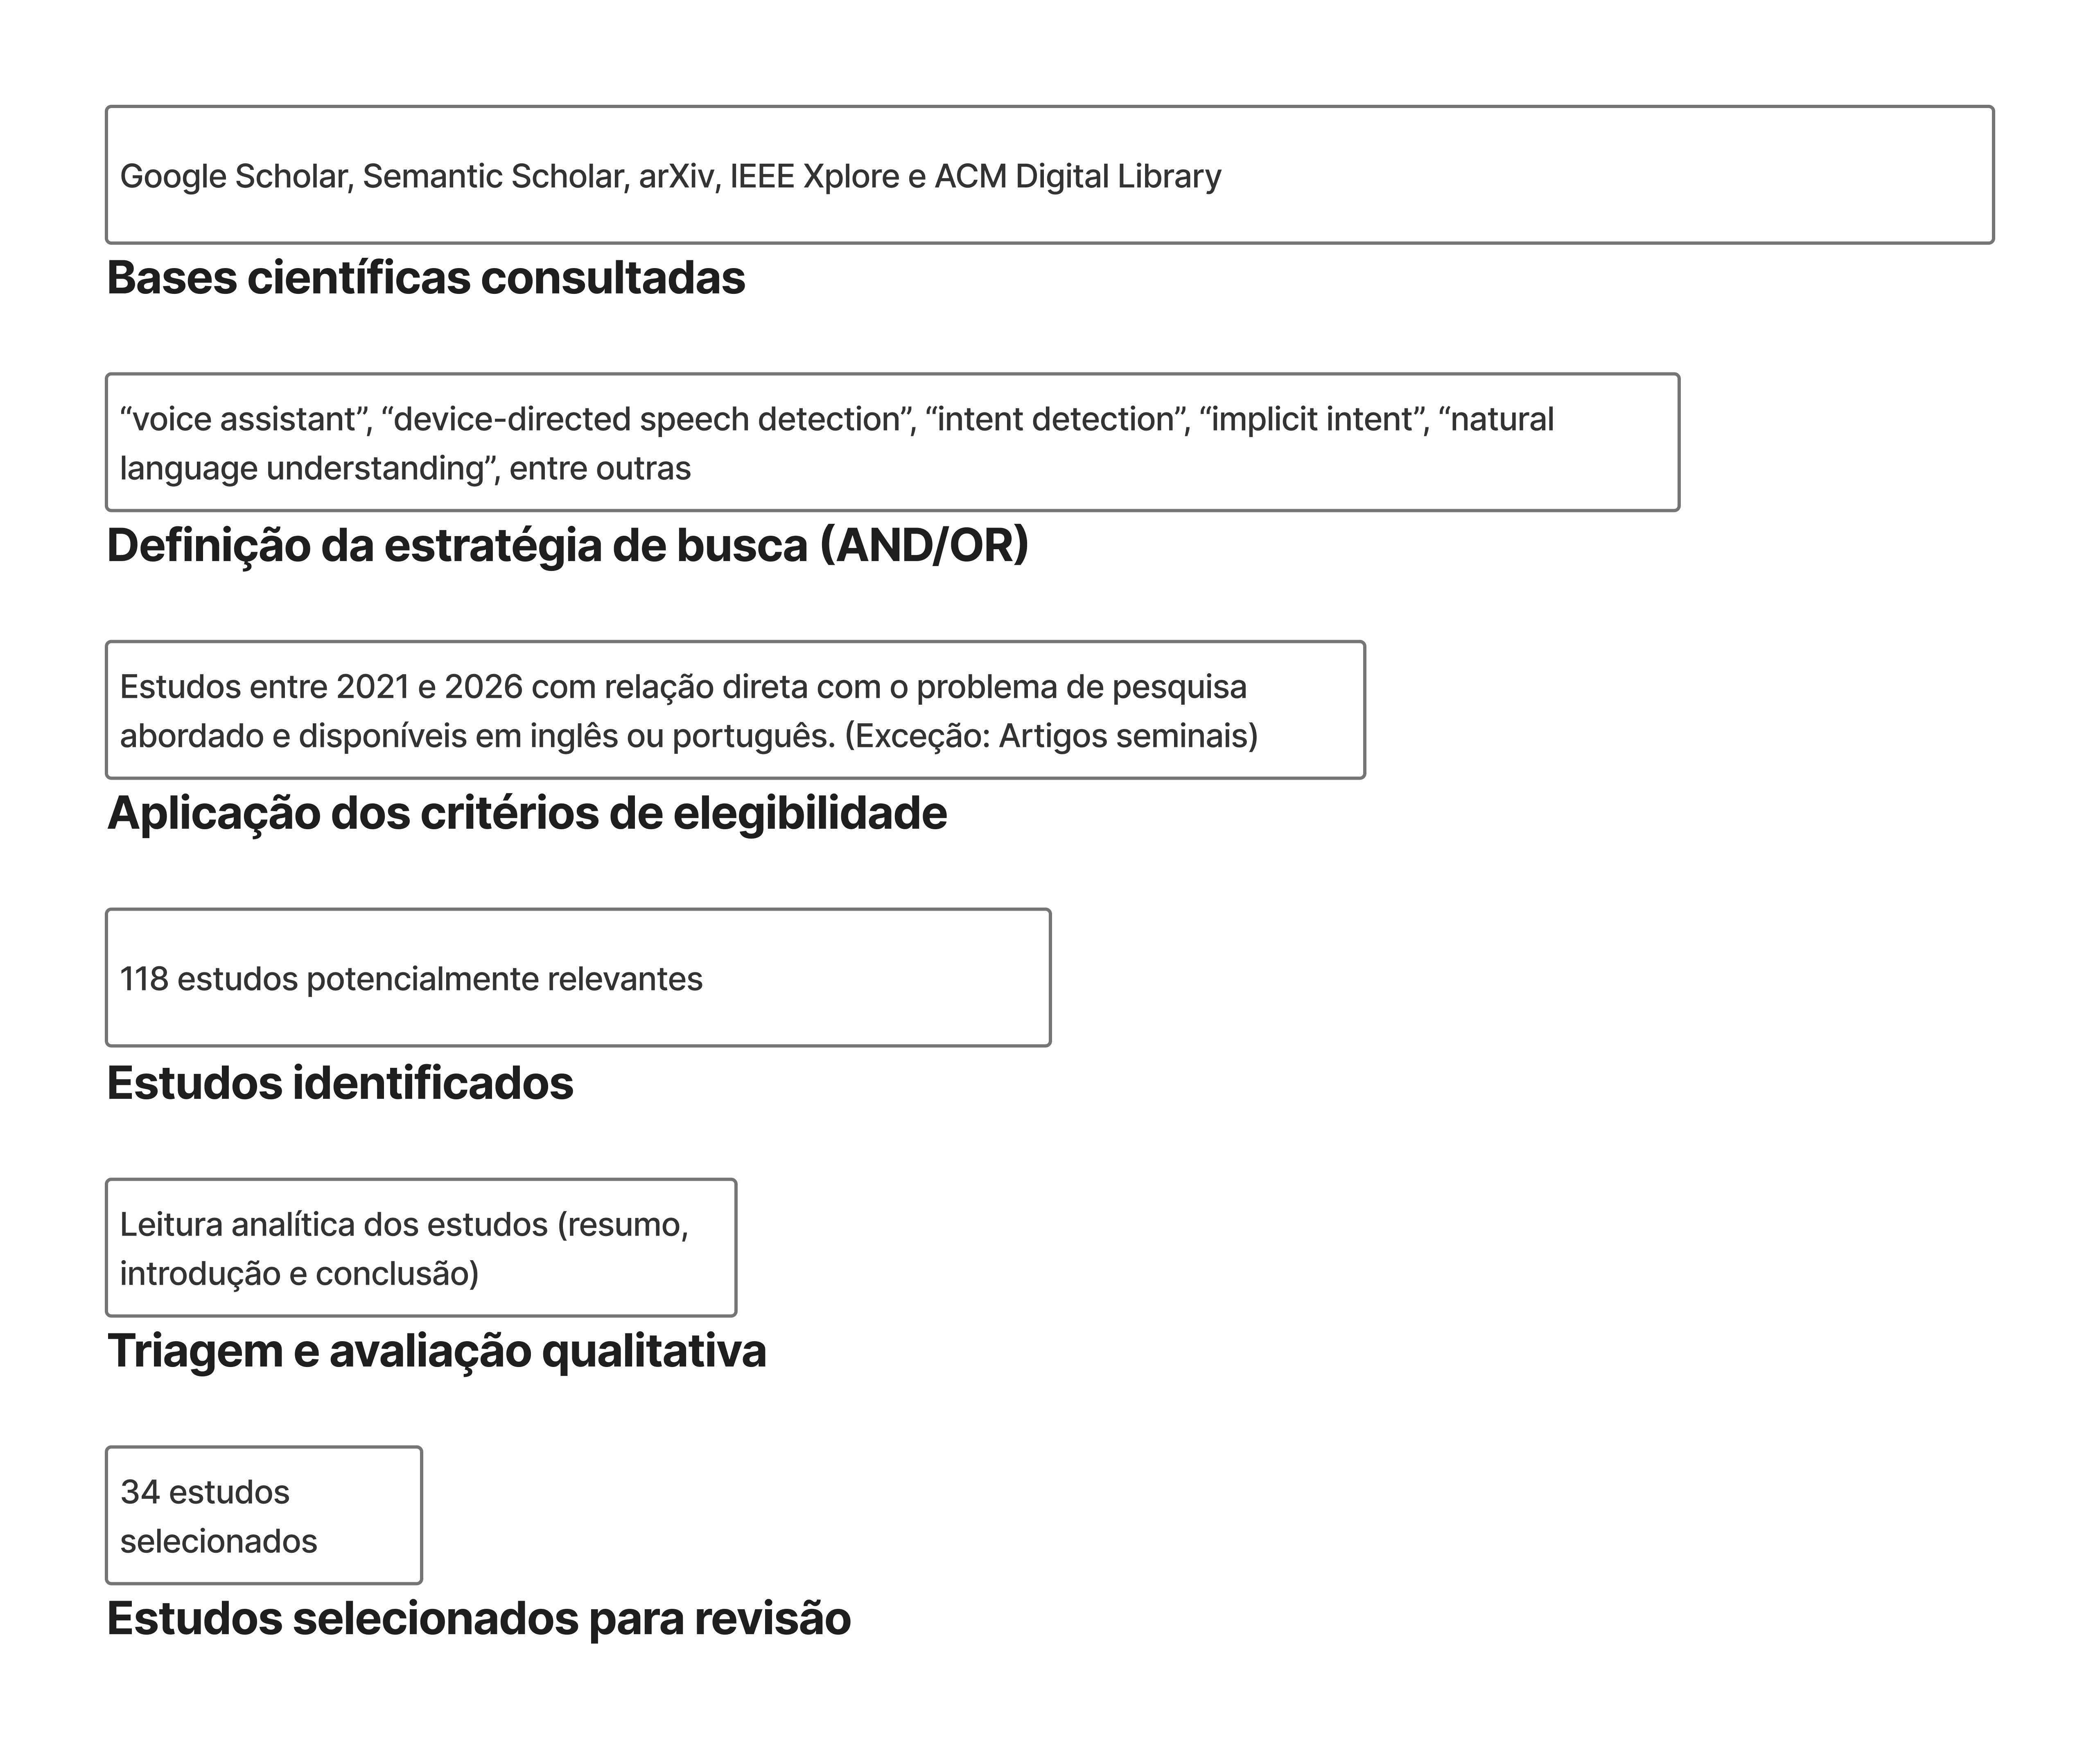
\includegraphics[width=0.85\textwidth]{funil.png} 
    \fonte{Elaborado pelo autor (2026).}
    \label{fig:funil}
\end{figure}

A pesquisa bibliográfica foi conduzida de forma estruturada com o objetivo de identificar trabalhos científicos relevantes sobre detecção de intenção em linguagem natural, assistentes virtuais baseados em voz, DDSD e técnicas de aprendizado de máquina aplicadas ao reconhecimento e classificação de comandos de voz.

Foram consultadas bases de dados acadêmicas amplamente utilizadas na área de Computação, incluindo Google Scholar, Semantic Scholar, arXiv, IEEE Xplore e ACM Digital Library. Essas plataformas foram selecionadas por concentrarem artigos científicos, pré-publicações e trabalhos revisados por pares com abrangência nas áreas de processamento de fala, linguagem natural e aprendizado de máquina.

As buscas utilizaram combinações de palavras-chave em inglês, tais como: \textit{``voice assistant''}, \textit{``device-directed speech detection''}, \textit{``intent detection''}, \textit{``keyword spotting''}, \textit{``implicit intent''}, \textit{``wake-word''}, \textit{``false trigger mitigation''}, \textit{``natural language understanding''} e \textit{``voice command classification''}. Essas expressões foram combinadas por meio de operadores booleanos (AND, OR) para ampliar ou restringir os resultados conforme necessário.

Como critérios de inclusão, foram considerados: (a) trabalhos publicados entre 2021 e 2026; (b) disponibilidade nos idiomas inglês ou português; (c) relação direta com o problema de pesquisa, priorizando-se artigos que apresentassem experimentos, métodos de classificação ou avaliações de sistemas de interação por voz. Como exceção, foram incluídos artigos seminais anteriores ao período definido, por representarem contribuições fundamentais para a área, como os trabalhos sobre a arquitetura Transformer \cite{Vaswani2017} e o BERT \cite{Devlin2019}.

Como critérios de exclusão, foram desconsiderados: (a) trabalhos publicados antes de 2021, exceto os seminais; (b) artigos sem relação direta com detecção de intenção, DDSD ou classificação de comandos de voz; (c) trabalhos duplicados entre as bases consultadas.

O processo de seleção ocorreu em duas etapas, conforme ilustrado na Figura~\ref{fig:funil}. Na triagem inicial, foram identificados 118 artigos potencialmente relevantes com base na leitura de título e resumo. Na etapa de afunilamento, a análise em maior profundidade resultou na seleção de 26 trabalhos para compor a fundamentação teórica, os trabalhos relacionados e as referências deste estudo. Adicionalmente, foram incluídos 7 artigos seminais anteriores a 2021, entre os quais se destacam os trabalhos sobre a arquitetura Transformer \cite{Vaswani2017}, o BERT \cite{Devlin2019}, o BERTimbau \cite{Souza2020} e os primeiros estudos de DDSD \cite{Mallidi2018, Norouzian2019}. Dessa forma, o conjunto final de referências selecionadas para este trabalho foi composto por 33 artigos.

% ---------------------------------------------------------------
\section{Referencial teórico}
\label{sec:referencial}

O referencial teórico apresenta os conceitos que sustentam este trabalho, estabelecendo um contraponto entre o modelo predominante de interação com assistentes virtuais baseado em comandos explícitos (\textit{wake-words}) e a busca por interações mais naturais por meio da DDSD. A organização dos tópicos segue o fluxo típico de processamento de um assistente virtual baseado em voz, desde a captura e identificação da fala destinada ao sistema, passando pela transcrição do áudio, até a compreensão semântica da intenção do usuário.

% ---------------------------------------------------------------

\subsection{Assistentes virtuais e interação por voz}

A evolução da Interação Humano-Computador (conhecida por HCI, do inglês \textit{Human-Computer Interaction}) tem avançado das interfaces puramente gráficas e táteis em direção a interfaces conversacionais e ubíquas. Nesse contexto, os assistentes virtuais baseados em voz consolidaram-se como agentes computacionais capazes de interpretar linguagem natural, processar requisições e executar tarefas automatizadas, mediando a relação entre o usuário e ecossistemas de serviços digitais.

De acordo com \citeonline{Jurafsky2024}, assistentes virtuais são sistemas que integram tecnologias de ASR (Reconhecimento Automático de Fala, do inglês \textit{Automatic Speech Recognition}), Compreensão de Linguagem Natural (NLU, do inglês \textit{Natural Language Understanding}) e Síntese de Fala (TTS, do inglês \textit{Text-to-Speech}) para viabilizar interações fluidas entre humanos e dispositivos. O funcionamento típico segue um \textit{pipeline} sequencial: (i)~captura do sinal de áudio; (ii)~Detecção de Atividade de Voz (VAD, do inglês \textit{Voice Activity Detection}); (iii)~ASR; (iv)~NLU; e (v)~geração da resposta ou execução da ação solicitada.

Na maioria dos sistemas comerciais, essas etapas são precedidas por um módulo de detecção de \textit{wake-word}, que atua como gatilho para iniciar o processamento mais custoso \cite{Garg2021}. Essa arquitetura permite que o assistente permaneça em modo de baixo consumo até ser explicitamente invocado. A relevância dessas tecnologias é corroborada pelo crescimento acelerado do mercado global de assistentes de voz, conforme apresentado no Capítulo~\ref{cap:introducao} \cite{NMSC2025}.

Para que a interação por voz funcione bem, o sistema precisa identificar quando uma fala é realmente direcionada a ele. No dia a dia, uma pessoa pode alternar entre conversar com outras pessoas e dar comandos ao dispositivo, e o assistente deve ser capaz de distinguir essas situações. Essa tarefa é especialmente importante em computadores pessoais, que costumam ser utilizados em ambientes compartilhados e nos quais conversas comuns podem ser confundidas com comandos. É essa distinção que orienta o presente

% ---------------------------------------------------------------

\subsection{Detecção de Atividade de Voz (VAD)}

A Detecção de Atividade de Voz (VAD) é a primeira etapa de processamento após a captura do áudio, sendo responsável por identificar os segmentos do sinal que contêm fala humana e separá-los de trechos de silêncio, ruído de fundo e sons não verbais \cite{Li2021}. Ao descartar trechos sem fala, o VAD reduz o volume de dados processado pelos módulos subsequentes (ASR e NLU), diminuindo o consumo computacional e a latência, aspectos críticos em dispositivos embarcados e de borda.

Em ambientes controlados, a tarefa é relativamente simples, baseada em limiares de energia ou características acústicas tradicionais. Em cenários reais, a robustez torna-se um desafio, e modelos baseados em aprendizado profundo têm alcançado resultados superiores \cite{Li2021}. A qualidade da detecção impacta diretamente as etapas posteriores do \textit{pipeline}. Um VAD muito permissivo gera ativações desnecessárias, enquanto um VAD restritivo demais pode descartar falas relevantes. Dessa forma, o equilíbrio entre sensibilidade e especificidade constitui um aspecto importante para o desempenho de assistentes de voz. Embora o VAD esteja fora do escopo de implementação deste trabalho, seu papel como pré-requisito funcional do \textit{pipeline} justifica sua menção no referencial.

% ---------------------------------------------------------------

\subsection{Reconhecimento Automático de Fala (ASR)}

O Reconhecimento Automático de Fala (ASR) consiste na conversão de um sinal de áudio contendo fala humana em texto legível por máquina \cite{Jurafsky2024}. No contexto de assistentes virtuais, o ASR atua como ponte entre o processamento do sinal acústico e os módulos de compreensão semântica.

Historicamente, os sistemas de ASR baseavam-se em abordagens híbridas que combinavam Modelos de Markov Ocultos (HMM, do inglês \textit{Hidden Markov Models}) com modelos de linguagem estatísticos \cite{Jurafsky2024}. Essas abordagens dominaram a área por décadas, mas apresentavam limitações na modelagem de dependências temporais longas e no aproveitamento de grandes volumes de dados. A partir da década de 2010, o aprendizado profundo trouxe avanços significativos, inicialmente com redes recorrentes (RNN, LSTM) e convolucionais, e posteriormente com a arquitetura Transformer \cite{Vaswani2017}, que permitiu saltos expressivos de desempenho. Modelos contemporâneos, como o Whisper \cite{Radford2023}, atingiram robustez elevada em múltiplos idiomas ao serem treinados com supervisão fraca em corpora massivos. Os detalhes técnicos do Whisper e de outros modelos de ASR empregados neste trabalho são apresentados na Seção~\ref{sec:fundamentos}.

A qualidade dos sistemas de ASR pode ser avaliada pela métrica \textit{Word Error Rate} (traduzida como Taxa de Erro de Palavras, referenciada pela sigla WER). Essa métrica mede a proporção de palavras substituídas, excluídas ou inseridas na transcrição em comparação com o texto de referência \cite{Jurafsky2024}. Em assistentes de voz, esses erros podem afetar as etapas seguintes do processamento, incluindo a classificação dos enunciados. Por isso, o WER é uma medida importante para entender como a qualidade da transcrição pode influenciar o desempenho geral do sistema.

% ---------------------------------------------------------------

\subsection{Wake-words: mecanismo, vantagens e limitações}

As \textit{wake-words} (também denominadas \textit{hotwords} ou palavras de ativação) constituem o mecanismo predominante de ativação em assistentes virtuais comerciais. Trata-se de expressões pré-definidas, tais como ``Hey Siri'', ``Alexa'', ``Ok Google'' e ``Hey Bixby'', que funcionam como gatilho para despertar o sistema do estado de espera e iniciar o processamento da solicitação do usuário \cite{Garg2021}.

Do ponto de vista técnico, a detecção de \textit{wake-words} é realizada por um módulo de \textit{keyword spotting} que opera continuamente no dispositivo com consumo energético reduzido. Esse módulo permanece ativo mesmo quando os componentes mais custosos do \textit{pipeline} (ASR e NLU) estão inativos, ativando-os somente após a detecção positiva da palavra de ativação \cite{Garg2021}.

Essa abordagem oferece vantagens relevantes. Do ponto de vista energético, é eficiente e adequada para dispositivos alimentados por bateria \cite{Shin2023}. Contribui também para a preservação da privacidade, uma vez que o processamento em nuvem só é iniciado após a ativação explícita \cite{Nie2021}. Além disso, minimiza o processamento desnecessário de áudio ambiente.

Apesar da sua ampla utilização, o mecanismo de \textit{wake-words} apresenta algumas limitações. Do ponto de vista da HCI, a necessidade de dizer uma palavra específica para iniciar a interação torna a comunicação menos natural em comparação com uma conversa entre pessoas \cite{Nie2021}. Além disso, esses sistemas podem ser ativados por engano quando alguém pronuncia palavras ou expressões semelhantes à palavra de ativação, fenômeno conhecido como \textit{FakeWake}. Em seu estudo, \citeonline{Chen2021} desenvolveram um método automático para gerar \textit{fuzzy words}, ou seja, expressões foneticamente semelhantes às palavras de ativação. Os autores identificaram 965 expressões capazes de ativar indevidamente oito modelos populares de auto-falantes inteligentes, em testes realizados em inglês e chinês. Esse tipo de falha pode prejudicar a experiência de uso e trazer riscos à privacidade.

Para mitigar os falsos gatilhos, foram propostas técnicas de mitigação de falsos acionamentos (FTM, do inglês \textit{False Trigger Mitigation}). \citeonline{Garg2021} apresentaram uma arquitetura baseada em Transformer com processamento em fluxo contínuo, capaz de suprimir até 95\% dos falsos positivos utilizando apenas um segundo de áudio contextual após a ativação. Apesar dos avanços, essas soluções adicionam complexidade ao sistema e não eliminam a necessidade de uma ativação explícita inicial, motivando o desenvolvimento de alternativas como a DDSD.

% ---------------------------------------------------------------

\subsection{Detecção de Fala Direcionada ao Dispositivo (DDSD)}

A Detecção de Fala Direcionada ao Dispositivo (DDSD) é definida como a tarefa de classificação binária que visa determinar automaticamente se um enunciado é intencionalmente direcionado a um assistente virtual ou se faz parte de uma conversa incidental entre humanos \cite{Mallidi2018, Wagner2024}.

Diferentemente do mecanismo de \textit{wake-words}, a DDSD busca permitir interações mais naturais, aproximando a comunicação humano-computador do padrão conversacional humano e superando as limitações de rigidez e fricção cognitiva discutidas na subseção anterior \cite{Nie2021}.

As pesquisas sobre DDSD têm seguido principalmente duas linhas: abordagens multimodais, que combinam diferentes tipos de informação, e abordagens unimodais, baseadas apenas em áudio ou texto. Entre as abordagens multimodais, \citeonline{Wagner2024} combinaram informações acústicas, sinais do decodificador do ASR e a transcrição textual em um único LLM (Modelo de Linguagem de Grande Porte, do inglês \textit{Large Language Model}). Os autores obtiveram uma redução relativa de até 39\% na taxa de erro igual em comparação com o modelo baseado apenas em texto e de até 61\% em relação ao modelo baseado apenas e áudio. \citeonline{Krishna2023}, por sua vez, combinaram informações verbais com características prosódicas, como entonação, ritmo e pausas, e observaram melhorias na taxa de falsa . aceitação. Já \citeonline{Nie2021} invetigaram uma abordagem para robôs de diálogo equipado com câmera, utilizando informações de áudio e vídeo para verificar se a fala vinha da pessoa posicionada diante do robô e a transcrição para identificar a intenção de interagir com o sistema. Entre as abordagens baseadas apenas em áudio, \citeonline{Norouzian2019} utilizaram características espectrais em conjunto com mecanismos de atenção para classificar os enunciados como direcionados ou não ao dispositivo.

Embora as abordagens multimodais possam apresentar melhores resultados em cenários complexos, elas exigem mais recursos computacionais, sincronização entre diferentes tipos de informação e grandes volumes de dados anotados. Esses requisitos podem dificultar sua implementação em dispositivos com capacidade computacional limitada \cite{Xu2024}.

Nesse cenário, pesquisas recentes têm explorado abordagens que utilizam apenas o texto das transcrições geradas por sistemas de ASR para identificar se uma fala é direcionada ao dispositivo. Embora essa alternativa ainda seja menos estudada do que as abordagens acústicas e multimodais, ela apresenta vantagens como uma arquitetura mais simples e a possibilidade de analisar separadamente as etapas de transcrição e classificação. Isso também pode facilitar sua aplicação em idiomas com poucos dados anotados, como o português brasileiro. Em um estudo anterior à popularização dos modelos pré-treinados, \citeonline{Mallidi2018} observaram que os comandos dirigidos ao dispositivo costumam ser mais curtos e estruturados, enquanto as conversas entre pessoas tendem a ser mais espontâneas e menos formais. Essas diferenças também podem aparecer nas transcrições geradas pelo ASR. Estudos mais recentes reforçam essa ideia ao mostrar que o conteúdo textual das transcrições fornece informações úteis para identificar se uma fala é direcionada ao dispositivo \cite{Wagner2024, Dighe2024}.

% ---------------------------------------------------------------

\subsection{Processamento de Linguagem Natural e classificação de intenção}

O Processamento de Linguagem Natural (do inglês \textit{Natural Language Processing}, referido pela sigla NLP) compreende o conjunto de técnicas computacionais destinadas à análise, compreensão e geração de linguagem humana em formato textual \cite{Jurafsky2024}. No contexto de assistentes virtuais, a subárea de Compreensão de Linguagem Natural (NLU) é responsável por extrair o significado semântico e a intenção do usuário a partir das transcrições geradas pelo ASR \cite{Weld2022}.

A partir de um enunciado do usuário, o sistema busca identificar a intenção da fala, ou seja, qual ação deve ser realizada \cite{Weld2022}. Essa tarefa pode ser combinada com o preenchimento de \textit{slots} (\textit{slot filling}), que consiste em identificar as informações necessárias para executar a ação. Por exemplo, no comando ``abre o YouTube e pesquisa receitas de bolo'', a intenção é realizar uma pesquisa, enquanto o termo ``receitas de bolo'' corresponde ao parâmetro de busca.

Historicamente, os sistemas de classificação de intenção baseavam-se em regras manuais e padrões lexicais. Métodos estatísticos, como Máquinas de Vetores de Suporte (SVM), tornaram-se predominantes na sequência \cite{Manning2008}. Foi, contudo, a partir da introdução da arquitetura Transformer \cite{Vaswani2017} e, especialmente, do modelo BERT \cite{Devlin2019} que a área experimentou avanço expressivo. Em levantamento abrangente, \citeonline{Weld2022} concluem que modelos pré-treinados baseados em Transformers superam consistentemente abordagens anteriores em tarefas de detecção de intenção, tanto em precisão quanto em generalização.

Uma das vantagens dos modelos pré-treinados é a possibilidade de ajustá-los por meio de \textit{fine-tuning} utilizando conjuntos relativamente pequenos de dados rotulados \cite{Devlin2019}. Isso é especialmente útil para idiomas que ainda possuem poucos recursos linguísticos disponíveis. No caso da DDSD textual, esses modelos são utilizados para uma etapa anterior à identificação da intenção: a partir da transcrição gerada pelo ASR, o sistema classifica o enunciado como direcionado ao computador (DD) ou não direcionado ao dispositivo (NDD), sem depender de uma \textit{wake-word} explícita.

\subsection{Modelos baseados em Transformers}

A arquitetura Transformer, proposta por \citeonline{Vaswani2017}, representou um dos principais marcos do NLP ao substituir recorrência e convoluções pelo mecanismo de \textit{atenção multi-cabeça} como principal componente para modelar dependências em sequências textuais. A partir dessa arquitetura, \citeonline{Devlin2019} propuseram o BERT (\textit{Bidirectional Encoder Representations from Transformers}), que introduziu o pré-treinamento bidirecional profundo e demonstrou ganhos expressivos em diversas tarefas de compreensão textual. O detalhamento técnico dessas arquiteturas, incluindo as formulações matemáticas do mecanismo de atenção e o processo de \textit{fine-tuning}, é apresentado na Seção~\ref{sec:fundamentos}.

Para o português brasileiro, \citeonline{Souza2020} desenvolveram o BERTimbau, um modelo BERT pré-treinado especificamente para o idioma. Os autores obtiveram resultados superiores aos de modelos multilíngues em tarefas como similaridade semântica, inferência textual e reconhecimento de entidades nomeadas. Outros modelos também foram desenvolvidos para o português, como o DeBERTinha \cite{Abonizio2023} e o Albertina \cite{Rodrigues2023, Santos2024}, que apresentam diferentes características em relação ao desempenho e ao custo computacional. Esses modelos são apresentados com mais detalhes na Seção~\ref{sec:fundamentos} e fazem parte dos classificadores avaliados neste trabalho.

% ---------------------------------------------------------------
\section{Fundamentos}
\label{sec:fundamentos}

Esta seção detalha as tecnologias, algoritmos e metodologias específicas que serão empregadas no desenvolvimento da solução proposta. Diferentemente do referencial teórico, que contextualiza os conceitos gerais da área, os fundamentos aprofundam os aspectos técnicos diretamente utilizados na implementação.

% ---------------------------------------------------------------

\subsection{Arquitetura Transformer}

A arquitetura Transformer, introduzida por \citeonline{Vaswani2017}, eliminou a dependência de recorrência e convoluções, substituindo-as pelo mecanismo de atenção como principal componente para modelagem de sequências. Diferentemente das RNNs (Redes Neurais Recorrentes, do inglês \textit{Recurrent Neural Networks}), que processam sequências de forma sequencial, o Transformer processa todos os elementos da entrada simultaneamente, permitindo alto grau de paralelização. Embora variantes como LSTM (Memória de Longo e Curto Prazo, do inglês \textit{Long Short-Term Memory}) e GRU (Unidade Recorrente com Portão, do inglês \textit{Gated Recurrent Unit}) atenuem parcialmente o problema de dissipação de gradientes das RNNs tradicionais, essas arquiteturas ainda enfrentam limitações em dependências muito longas, que o Transformer supera por construção \cite{Vaswani2017}.

O componente central é o mecanismo de \textit{Self-Attention}. Para cada token da sequência, o modelo calcula três vetores: \textit{Query} (Q), \textit{Key} (K) e \textit{Value} (V). A atenção é obtida por:

\[
\text{Attention}(Q, K, V) = \text{softmax}\left(\frac{QK^T}{\sqrt{d_k}}\right)V
\]

onde \(d_k\) é a dimensão dos vetores de chave. Essa operação permite que cada token pondere a importância de todos os demais tokens da sequência. O fator de escala \(\sqrt{d_k}\) estabiliza os gradientes durante o treinamento.

Para aumentar a capacidade representacional, \citeonline{Vaswani2017} propuseram o \textit{Multi-Head Attention}, que executa o mecanismo de atenção em paralelo \(h\) vezes (tipicamente 8 ou 16 cabeças), cada uma com projeções lineares independentes de Q, K e V. As saídas são concatenadas e projetadas linearmente, permitindo que o modelo capture diferentes tipos de relações semânticas e sintáticas em uma mesma camada.

Como o Transformer não possui recorrência, é necessário injetar informação posicional por meio do \textit{Positional Encoding}. Os autores utilizaram funções seno e cosseno de diferentes frequências:

\[
PE_{(pos,2i)} = \sin\left(\frac{pos}{10000^{2i/d_{model}}}\right), \quad PE_{(pos,2i+1)} = \cos\left(\frac{pos}{10000^{2i/d_{model}}}\right)
\]

Esses valores são somados aos \textit{embeddings} dos tokens de entrada, fornecendo informação explícita sobre a ordem dos elementos.

A arquitetura completa é composta por blocos de \textit{Encoder} e \textit{Decoder}. Cada bloco do Encoder contém uma camada de Multi-Head Self-Attention seguida de uma rede \textit{feed-forward} posicionada (duas camadas lineares com ativação ReLU). O Decoder possui uma camada adicional de \textit{Cross-Attention} que recebe as saídas do Encoder. Conexões residuais e normalização de camada (\textit{layer normalization}) são aplicadas em torno de cada subcamada, facilitando o treinamento de redes profundas.

Para ilustrar: na frase ``O gato está no tapete'', o token ``tapete'' deve apresentar forte atenção com ``gato'' para capturar a relação semântica. Enquanto RNNs tradicionais processam a frase de forma sequencial, com dificuldade crescente para reter contextos distantes, mesmo com mecanismos de \textit{gating}, o Transformer relaciona ``tapete'' diretamente com ``gato'' em uma única passada, independentemente da distância entre eles.

A arquitetura serviu de base para modelos como BERT (apenas Encoder), GPT (apenas Decoder) e T5 (Encoder-Decoder), consolidando-se como o alicerce dos modernos Modelos de Linguagem de Grande Porte (LLMs).

% ---------------------------------------------------------------

\subsection{BERT e o mecanismo de fine-tuning}

O modelo BERT (\textit{Bidirectional Encoder Representations from Transformers}), proposto por \citeonline{Devlin2019}, introduziu o conceito de pré-treinamento bidirecional profundo. Diferentemente dos modelos anteriores, que processavam o texto de forma unidirecional, o BERT considera o contexto completo de cada palavra, analisando simultaneamente os tokens à esquerda e à direita.

O pré-treinamento ocorre por meio de duas tarefas em grandes corpora não anotados:

\begin{enumerate}
    \item \textbf{Masked Language Modeling (MLM)}: 15\% dos tokens da entrada são aleatoriamente mascarados, e o modelo deve prever o token original com base no contexto bidirecional. Na frase ``O [MASK] está no tapete'', o modelo aprende a prever ``gato'' considerando tanto o contexto anterior quanto o posterior.
    \item \textbf{Next Sentence Prediction (NSP)}: o modelo recebe pares de sentenças e deve identificar se a segunda é a continuação lógica da primeira, desenvolvendo compreensão de relações discursivas e coerência textual.
\end{enumerate}

Após o pré-treinamento, o BERT pode ser adaptado para tarefas específicas por meio de \textit{fine-tuning}. Nesse estágio, o modelo é inicializado com os pesos pré-treinados e continua o treinamento em um conjunto de dados menor e rotulado. Uma camada de classificação é adicionada sobre a representação do token especial \texttt{[CLS]}, que concentra informações de toda a sequência \cite{Devlin2019}. Os pesos das camadas anteriores também são atualizados, permitindo que as representações internas se ajustem à tarefa em questão.

Uma das vantagens do \textit{fine-tuning} é a necessidade de relativamente poucos dados rotulados e poucas épocas de treinamento. \citeonline{Devlin2019} demonstraram que, com essa abordagem, o BERT superou o estado da arte em 11 tarefas de NLP, incluindo os \textit{benchmarks} GLUE, SQuAD e SWAG.

Na classificação de enunciados, o processo é direto: a última camada é substituída por uma camada linear com \textit{softmax}, e o modelo é treinado minimizando a perda de entropia cruzada. Essa abordagem será aplicada ao BERTimbau, à DeBERTinha e à Albertina para especializá-los na tarefa de DDSD em português brasileiro.

% ---------------------------------------------------------------

\subsection{BERTimbau: BERT para o português brasileiro}

O BERTimbau, proposto por \citeonline{Souza2020}, é a versão do BERT pré-treinada especificamente para o português brasileiro. Seu desenvolvimento partiu da constatação de que modelos multilíngues, apesar do bom desempenho geral, apresentam limitações quando aplicados a idiomas com características morfossintáticas e vocabulário específicos.

O BERTimbau foi pré-treinado com aproximadamente 2,7 bilhões de tokens do corpus brWaC (\textit{Brazilian Web as Corpus}), composto por páginas da \textit{web} brasileira. O modelo foi disponibilizado em duas versões: BERTimbau Base, com 12 camadas e 110 milhões de parâmetros, e BERTimbau Large, com 24 camadas e 335 milhões de parâmetros \cite{Souza2020}.

O pré-treinamento seguiu a mesma metodologia do BERT original (MLM e NSP), porém, por ter sido treinado exclusivamente com dados em português brasileiro, o modelo desenvolveu representações mais adequadas às particularidades do idioma, tais como conjugações verbais complexas, artigos definidos e contrações comuns (``do'', ``na'', ``pelo'').

\citeonline{Souza2020} compararam o desempenho do BERTimbau com o do BERT multilíngue (mBERT) em diferentes tarefas de NLP para o português. O BERTimbau apresentou resultados superiores em todas as tarefas avaliadas: similaridade semântica, inferência textual e reconhecimento de entidades nomeadas. Nesta última, a diferença na pontuação F1 foi superior a cinco pontos percentuais. A disponibilização do modelo também facilitou o acesso a recursos de NLP adaptados ao português, reduzindo a necessidade de utilizar modelos multilíngues com desempenho inferior ou treinar modelos desde o início.

% ---------------------------------------------------------------

\subsection{DeBERTa, DeBERTinha e Albertina PT-BR}

Embora o BERT tenha estabelecido um novo patamar para modelos de linguagem, arquiteturas subsequentes buscaram superar suas limitações, especialmente quanto à representação de dependências sintáticas e à eficiência computacional. Destaca-se a família DeBERTa (\textit{Decoding-enhanced BERT with Disentangled Attention}), proposta por \citeonline{He2021}.

A principal inovação do DeBERTa é o mecanismo de atenção desentrelada (\textit{Disentangled Attention}). Enquanto o BERT representa cada token por um único vetor que combina informação de conteúdo e posição, o DeBERTa separa essas dimensões. Para cada par de tokens, a atenção é calculada considerando conteúdo e posição relativa de forma independente, o que permite modelagem mais precisa de relações sintáticas. Além disso, o DeBERTa utiliza um decodificador aprimorado (\textit{enhanced mask decoder}) durante o pré-treinamento \cite{He2021}.

Para o português brasileiro, \citeonline{Abonizio2023} desenvolveram a \textbf{DeBERTinha}, um modelo compacto baseado no DeBERTaV3 XSmall. O modelo utiliza um vocabulário adaptado ao português e foi pré-treinado com os corpora Carolina e brWaC. Com cerca de 40 milhões de parâmetros, a DeBERTinha foi avaliada em três tarefas: reconhecimento de entidades nomeadas, análise de sentimentos e similaridade entre sentenças. Os resultados mostraram que o modelo superou o BERTimbau Large em duas dessas tarefas \cite{Abonizio2023}.

Outra iniciativa importante é a família de modelos \textbf{Albertina PT-\*}, desenvolvida por \citeonline{Rodrigues2023}, com versões para o português europeu (PT-PT) e o português brasileiro (PT-BR). O modelo original possui cerca de 900 milhões de parâmetros e foi desenvolvido a partir da continuação do pré-treinamento do DeBERTa XLarge, alcançando resultados de destaque em tarefas de compreensão de linguagem em português. Posteriormente, \citeonline{Santos2024} ampliaram essa família com duas versões: uma com 1,5 bilhão de parâmetros, voltada ao desempenho, e outra com 100 milhões de parâmetros, que prioriza a eficiência computacional. A versão menor para o português brasileiro utiliza o DeBERTa Base como ponto de partida e foi pré-treinada com a parte brasileira do corpus OSCAR.

% ---------------------------------------------------------------

\subsection{Modelos baseline: TF-IDF, SVM e Regressão Logística}

Na classificação textual, é prática comum utilizar modelos mais simples e interpretáveis como \textit{baselines} para comparação com abordagens de \textit{deep learning}. Foram selecionados três componentes clássicos: TF-IDF para representação vetorial, combinado com SVM e Regressão Logística como classificadores.

A Frequência do Termo-Inverso da Frequência nos Documentos (TF-IDF, do inglês \textit{Term Frequency-Inverse Document Frequency}) é uma das técnicas mais tradicionais de representação vetorial de texto \cite{Manning2008}. Atribui pesos às palavras considerando a frequência do termo no documento (TF) e a raridade do termo na coleção (IDF):

\[
\text{TF-IDF}(t,d) = \text{TF}(t,d) \times \log\left(\frac{N}{\text{DF}(t) + 1}\right)
\]

onde \( t \) é o termo, \( d \) é o documento, \( N \) é o número total de documentos e \( \text{DF}(t) \) é o número de documentos que contêm \( t \). Essa ponderação reduz o peso de termos comuns e aumenta o peso de termos discriminativos.

As Máquinas de Vetores de Suporte (SVM), propostas por \citeonline{Cortes1995}, buscam o hiperplano que maximiza a margem de separação entre as classes. Em problemas não linearmente separáveis, o truque do kernel (\textit{kernel trick}) mapeia os dados para um espaço de maior dimensionalidade onde a separação linear se torna possível. Na classificação binária de DDSD (DD~$\times$~NDD), o SVM busca maximizar a distância entre os vetores TF-IDF das duas classes.

A Regressão Logística modela a probabilidade de uma classe binária por meio da função sigmoide:

\[
P(y=1|x) = \frac{1}{1 + e^{-(\beta_0 + \beta_1 x_1 + \dots + \beta_n x_n)}}
\]

Apesar de ser um modelo linear, a Regressão Logística frequentemente obtém bom desempenho em classificação textual quando combinada com TF-IDF, especialmente em conjuntos de dados de tamanho moderado \cite{Manning2008}.

Ambos os classificadores são amplamente utilizados como \textit{baselines} em pesquisas de NLP por serem eficientes, interpretáveis e constituírem referência sólida para aferir o ganho real obtido por modelos mais complexos. A comparação entre os \textit{baselines} TF-IDF+SVM e TF-IDF+LR e os classificadores baseados em Transformer permitirá quantificar objetivamente o ganho da abordagem baseada em Transformer na tarefa de DDSD.

% ---------------------------------------------------------------

\subsection{ASR com Whisper}

O Whisper é um modelo de ASR de grande escala desenvolvido pela OpenAI \cite{Radford2023}. Diferentemente da maioria dos sistemas tradicionais, treinados com supervisão forte em conjuntos relativamente pequenos e limpos, o Whisper foi treinado com supervisão fraca em um corpus de aproximadamente 680 mil horas de áudio multilíngue coletado da web. Essa estratégia conferiu ao modelo alta robustez e capacidade de generalização.

Arquiteturalmente, o Whisper segue o padrão Encoder-Decoder baseado em Transformer. O \textit{encoder} processa o espectrograma log-Mel do áudio de entrada, gerando representações contextuais. O \textit{decoder}, autoregressivo, gera o texto transcrito token a token, podendo também realizar tarefas como tradução de fala e identificação de idioma por meio de \textit{prompts} especiais \cite{Radford2023}.

em 2024, a OpenAI lançou o Whisper Large V3 Turbo, uma versão que reduz o número de camadas do \textit{decoder} de 32 para 4. Essa mudança torna a transcrição mais rápida, mantendo um desempenho próximo ao do modelo completo, o que favorece seu uso em aplicações que precisam processar áudio com baixa latência \cite{OpenAI2024Turbo}.

Entre as vantagens do Whisper para este trabalho destacam-se o bom desempenho em português brasileiro, a robustez a ruídos ambientais e a capacidade nativa de identificação de idioma. As transcrições geradas servirão de entrada para o classificador textual de DDSD. Experimentos no TCC2 incluirão a comparação entre diferentes tamanhos de modelo (Medium, Large V3 e Turbo) e a análise da relação entre o WER do ASR e o desempenho do classificador.

Embora o Whisper represente o estado da arte em ASR multilíngue, erros de transcrição podem ocorrer, especialmente em ambientes ruidosos ou com vocabulário incomum. A avaliação do impacto desses erros sobre a detecção do direcionamento da fala constitui um dos objetivos específicos deste trabalho.

% ---------------------------------------------------------------

\subsection{Métricas de avaliação}
\label{sec:metricas}

A avaliação de modelos de classificação em tarefas de DDSD requer métricas que analisem não apenas a acurácia geral, mas também o equilíbrio entre erros de falso positivo e falso negativo. Serão utilizadas métricas tradicionais de classificação binária e métricas específicas da área.

A \textbf{Acurácia} (\textit{Accuracy}) mede a proporção de classificações corretas em relação ao total de amostras. Embora intuitiva, pode ser enganosa em conjuntos desbalanceados, situação comum em DDSD, onde falas não direcionadas ao dispositivo geralmente são mais frequentes \cite{Manning2008}.

A \textbf{Precisão} (\textit{Precision}) indica a proporção de exemplos classificados como positivos que são realmente positivos. Representa, neste contexto, a proporção de falas classificadas como direcionadas ao dispositivo que efetivamente o eram. É especialmente relevante quando o custo de falsos positivos (ativações indesejadas) é alto \cite{Manning2008}.

A \textbf{Sensibilidade} (\textit{Recall}) mede a proporção de exemplos positivos corretamente identificados. Um \textit{recall} baixo indica que muitos comandos do usuário estão sendo ignorados \cite{Manning2008}.

O \textbf{F1-Score} representa a média harmônica entre Precisão e Sensibilidade:

\[
F1 = 2 \times \frac{\text{Precision} \times \text{Recall}}{\text{Precision} + \text{Recall}}
\]

No cenário de DDSD, o F1-Score é uma das métricas principais, pois reflete o compromisso entre ativações corretas e ativações indevidas.

A \textbf{Taxa de Erro Igual} (EER, do inglês \textit{Equal Error Rate}) corresponde ao ponto na curva ROC onde a taxa de falsos positivos iguala a taxa de falsos negativos. Quanto menor o EER, melhor o desempenho do sistema. \citeonline{Mallidi2018} e \citeonline{Wagner2024} adotam o EER como métrica principal, pois ele resume o desempenho do sistema sem exigir a escolha prévia de um \textit{threshold} de decisão.

Será calculada também a \textbf{Área sob a Curva ROC (ROC-AUC)}, que avalia a capacidade discriminativa do modelo em diferentes \textit{thresholds}. Por fim, como o sistema proposto utiliza transcrições de ASR, o impacto da qualidade da transcrição será analisado por meio da \textbf{Word Error Rate (WER)}. Estudos demonstram correlação direta entre o WER do ASR e a degradação do desempenho do classificador textual \cite{Dighe2024}.

A combinação dessas métricas permite avaliação multidimensional: acurácia geral, equilíbrio entre precisão e \textit{recall}, robustez a variações de \textit{threshold} (EER) e sensibilidade à qualidade da transcrição (WER). Todas serão calculadas com validação cruzada e conjuntos de teste separados, assegurando maior confiabilidade dos resultados.

% ---------------------------------------------------------------\

\section{Trabalhos relacionados}
\label{sec:trabalhos_relacionados}

Nesta seção, são apresentados e discutidos os principais estudos sobre DDSD, selecionados a partir da metodologia descrita na Seção~\ref{sec:metodologia_pesquisa}.

Os trabalhos foram selecionados segundo dois critérios centrais: (i) abordagem direta do problema de DDSD ou de tarefa funcionalmente equivalente, isto é, a classificação automática de enunciados como dirigidos ou não a um sistema computacional, e (ii) uso de componente textual ou acústico relevante para a decisão de direcionamento. Trabalhos que tratam apenas de ASR, VAD, \textit{keyword spotting} clássico ou classificação de intenção em domínios distintos foram excluídos, pois não compartilham o problema central investigado neste TCC \cite{Wazlawick2020}.

Com base nesses critérios, três trabalhos foram selecionados como relacionados principais. O primeiro, de \citeonline{Mallidi2018}, é um dos primeiros estudos de DDSD voltados a assistentes de voz comerciais e já combinava áudio e texto. O segundo, de \citeonline{Wagner2024}, foi selecionado por representar uma das abordagens multimodais mais recentes encontradas na literatura revisada. O terceiro, de \citeonline{Dighe2024}, é o trabalho metodologicamente mais próximo desta proposta, por aplicar um modelo de linguagem sobre as saídas textuais do ASR na tarefa de DDSD. A análise crítica desses três estudos, conduzida nas subseções seguintes, permite identificar as lacunas que este trabalho busca preencher.

% ---------------------------------------------------------------

\subsection{Mallidi et al. (2018)}

O trabalho de \citeonline{Mallidi2018}, intitulado \textit{Device-directed Utterance Detection}, foi publicado por pesquisadores da Amazon nos anais do \textit{*Interspeech*} em 2018. Os autores mencionam pesquisas anteriores que utilizavam características prosódicas e escores de confiança do ASR para identificar falas direcionadas ao dispositivo. O estudo se destaca por aplicar redes neurais profundas à DDSD no contexto de assistentes de voz comerciais. Além disso, os autores utilizaram a classificação binária e a taxa de erro igual (EER) para avaliar o desempenho do sistema, uma abordagem também adotada em trabalhos posteriores \cite{Wagner2024}.

O estudo parte de um problema comum no uso de assistentes de voz. Dispositivos como Amazon Echo e Google Home podem captar falas de várias pessoas e sons de televisores, especialmente em ambientes como salas de estar. Por isso, precisam distinguir os comandos direcionados a eles das conversas e dos demais sons do ambiente. \citeonline{Mallidi2018} destacam duas aplicações para esse tipo de classificador: evitar ativações acidentais e permitir que o usuário faça pedidos de continuação sem precisar repetir a \textit{wake-word}. Por exemplo, após dizer ``Computador, tocar música'', o usuário poderia simplesmente pedir ``abaixar o volume'' \cite{Mallidi2018}.

O modelo utiliza três fontes de informação para classificar os enunciados. A primeira é uma representação do áudio (\textit{embedding} acústico), gerada por uma rede LSTM a partir de energias de bancos de filtros em escala logarítmica (LFBEs). A segunda é uma representação textual da transcrição mais provável do ASR (1-best), obtida por uma LSTM em nível de caracteres (\textit{Char LSTM}). Essa rede recebe a sequência de vetores de palavras da transcrição, gerados a partir de representações pré-treinadas com GloVe. A terceira fonte corresponde a características extraídas do decodificador do ASR. Por fim, as três representações são concatenadas e enviadas a uma rede neural \textit{feed-forward}, que produz a classificação final do enunciado \cite{Mallidi2018}.

Os experimentos foram realizados com gravações reais de interações com dispositivos de campo distante, em inglês. O conjunto de dados continha 350 mil enunciados (250 horas de áudio) para treinamento e 50 mil enunciados (30 horas) para teste. Quando avaliadas separadamente, as características do decodificador do ASR apresentaram EER de 9,3\%, o \textit{embedding} acústico obteve 10,9\% e o \textit{embedding} da transcrição alcançou 20,1\%. Ao combinar as três fontes de informação, os autores reduziram o EER para 5,2\%, uma melhora relativa de 44\% em comparação com o melhor resultado individual \cite{Mallidi2018}.

Ao analisar as transcrições, \citeonline{Mallidi2018} observaram que os comandos direcionados ao dispositivo tendem a ser mais curtos e estruturados, enquanto as conversas entre pessoas costumam ser mais espontâneas e apresentar construções menos formais. Os autores também verificaram que essas diferenças podem ser percebidas nas transcrições geradas pelo ASR \cite{Mallidi2018}. Essa constatação reforça a ideia de que o próprio texto pode fornecer informações úteis para identificar se uma fala é direcionada ao dispositivo.

Apesar da contribuição do estudo, a abordagem baseada apenas em texto apresentou o pior resultado entre as fontes de informação avaliadas individualmente. O modelo utilizado era uma LSTM em nível de caracteres, baseada em representações estáticas, desenvolvidas antes da popularização dos Transformers pré-treinados, como o BERT \cite{Devlin2019}. Modelos dessa família trouxeram avanços em tarefas de classificação de texto \cite{Weld2022}, o que abre espaçopara investigar seu desempenho na DDSD. Além disso, os experimentos de \citeonline{Mallidi2018} foram realizados apenas em inglês e utilizaram dados proprietários, o que limita a avaliação dos resultados em outros idiomas, como o português brasileiro.

O trabalho de \citeonline{Mallidi2018} contribui para esta pesquisa ao apresentar a DDSD como um problema de classificação binária entre enunciados direcionados ao dispositivo (DD) e não direcionados (NDD), utilizar o EER como métrica de avaliação e mostrar que as transcrições contêm informações úteis para essa tarefa. A principal diferença está na abordagem adotada: enquanto os autores combinam informações de áudio, do texto e do decodificador do ASR, este trabalho utiliza apenas o texto das transcrições e investiga o desempenho de modelos pré-treinados para o português brasileiro.

% ---------------------------------------------------------------

\subsection{Wagner et al. (2024)}

O trabalho de \citeonline{Wagner2024}, intitulado \textit{A Multimodal Approach to Device-Directed Speech Detection with Large Language Models}, foi publicado em 2024 no IEEE \textit{International Conference on Acoustics, Speech and Signal Processing} (ICASSP), por pesquisadores da Apple e da Technische Hochschule Nürnberg. O estudo investiga como permitir que assistentes virtuais reconheçam comandos direcionados a eles sem exigir que o usuário diga uma palavra ou frase de ativação antes de cada interação.

Os autores comparam três abordagens para detectar falas direcionadas ao dispositivo: modelos que utilizam apenas informações acústicas, LLMs que recebem transcrições e sinais do decodificador do ASR e um modelo multimodal que combina essas informações em um único LLM. Na abordagem multimodal, o áudio é representado por um \textit{embedding} extraído do \textit{encoder} do Whisper ou do CLAP. Além disso, são utilizados quatro sinais do decodificador do ASR: custo do grafo, custo acústico, confiança média por palavra e número médio de alternativas por palavra. Pequenas redes neurais \textit{feed-forward} transformam essas informações em vetores, que são combinados com a transcrição mais provável (1-best) e enviados ao GPT-2. O modelo, então, classifica o enunciado com uma resposta ``sim'' ou ``não'' \cite{Wagner2024}.

A maior parte dos experimentos utilizou o GPT-2 \textit{small}, com 124 milhões de parâmetros, escolhido por ser mais leve e adequado à execução em dispositivos com recursos limitados, como \textit{smartphones}. Nos experimentos finais, os autores também avaliaram uma versão do GPT-2 com 1,5 bilhão de parâmetro, ajustada por meio do LoRA (\textit{Low-Rank Adaptation}).

O treinamento utilizou cerca de 80 mil enunciados, divididos igualmente entre falas direcionadas e não direcionadas ao dispositivo. Em parte dos experimentos, os autores também incluíram transcrições adicionais sem o áudio correspondente. A avaliação foi realizada com aproximadamente 37 mil enunciados de bases de dados internas. Entre os modelos avaliados individualmente, a abordagem baseada apenas em texto obteve EER de 12,15\%, enquanto os modelos acústicos alcançaram 10,98\% com o Whisper e 19,13\% com o CLAP. Ao combinar as diferentes fontes de informação e ajustar completamente o GPT-2 \textit{small}, o melhor sistema multimodal, baseado no CLAP, atingiu EER de 7,45\%. Esse resultado representa um redução relativa de até 39\% em relação ao modelo textual e de até 61\% em relação ao modelo acústico. No caso do modelo GPT-2 com 1,5 bilhão de parâmetros, o sistema multimodal baseado no Whisper reduziu o EER de 7,95\% para 6,53\%, uma melhora relativa de aproximadamente 18\% e o melhor resultado geral do estudo \cite{Wagner2024}.

Os resultados mostram que a transcrição, por si só, já permite identificar muitos dos enunciados direcionados ao dispositivo, com um EER próximo ao do melhor modelo baseado apenas em áudio. No entanto, a combinação com informações acústicas e sinais do decodificador melhora o desempenho. Apesar desses resultados, a abordagem multimodal depende de recursos que podem dificultar sua reprodução em outros ambientes, como um \textit{encoder} de áudio, informações internas do decodificador do ASR e grandes volumes de áudio rotulados, disponíveis em bases privadas da empresa. Além disso, o artigo não especifica o idioma dos dados utilizados nem apresenta medições de latência ou consumo de memória \cite{Wagner2024}.

Neste trabalho, o estudo contribui de duas formas. A primeira é apresentar evidências recentes de que a transcrição gerada pelo ASR contém informações relevantes para a DDSD quando analisadas por um modelo de linguagem, o que dá suporte à hipótese de pesquisa deste TCC. A segunda é fornecer valores de EER que podem ser usados como referência aproximada, considerando as diferenças de idioma, corpus e modalidade entre os estudos. Assim, a abordagem proposta neste trabalho se aproxima do componente textual de \citeonline{Wagner2024}, mas é aplicada ao português brasileiro, utiliza dos modelos pré-treinados nesse idioma e não depende de sinais internos do ASR. 

% ---------------------------------------------------------------

\subsection{Dighe et al. (2024)}

O trabalho de \citeonline{Dighe2024}, intitulado \textit{Leveraging Large Language Models for Exploiting ASR Uncertainty}, também foi publicado no IEEE ICASSP em 2024 e é o estudo metodologicamente mais próximo desta proposta. Os autores investigam como LLMs podem lidar com os erros do ASR em tarefas de classificação sobre fala, e uma das tarefas avaliadas é a própria DDSD.

A proposta parte da observação de que os \textit{pipelines} tradicionais utilizam apenas a transcrição mais provável do ASR (1-best), descartando as hipóteses alternativas geradas pelo \textit{beam search}, que ajudam a representar a incerteza do reconhecimento. Como o WER dificilmente é zero em condições reais, os erros presentes na transcrição podem comprometer a classificação realizada pelo LLM \cite{Dighe2024}. Para reduzir esse problema, os autores fornecem ao modelo uma lista com hipóteses de transcrição mais prováveis (\textit{n-best-list}), acompanhada de um \textit{prompt} que explica como essas alternativas devem ser interpretadas. Além disso, ajustam o LLM por meio da técnica LoRA.

Os autores utilizaram o Vicuna-7B e avaliaram seu desempenho em duas tarefas: DDSD, com um base interna em inglês, e \textit{keyword spotting}, utilizando a base pública do Google Speech Commands. Na DDSD, o uso de uma lista com oito hipóteses de transcrição reduziu a taxa de falsos positivos de 8,3\% para 4,7\%, em comparação com a abordagem baseada apenas na transcrição mais provável (1-best). A taxa de verdadeiros positivos também aumentou ligeiramente, passando de 90,5\% para 91,8\%. Ao adaptar o modelo para gerar um escore de classificação, os autores obtiveram um EER de 7,4\% com 16 hipóteses. Esse resultado, porém, ficou acima dos 6,4\% alcançados pelo \textit{baseline} especializado LatticeRNN, que utiliza os reticulados do ASR. Na tarefa de \textit{keyword spotting}, a acurácia aumentou de 97,0\% para 97,5\% \cite{Dighe2024}.

O estudo demonstra que a combinação de ASR com um modelo de linguagem em uma arquitetura em cascata é viável para a DDSD e destaca a influência da qualidade da transcrição no desempenho da classificação. No entanto, os autores não apresentam uma avaliação do WER dos dados utilizados nem quantificam a relação entre os erros de transcrição e o desempenho do classificador. Essa lacuna fundamenta o terceiro objetivo específico deste TCC, que busca analisar a correlação entre o WER e a queda de desempenho do classificador no português brasileiro.

Outro ponto importante é o custo computacional dos modelos utilizados. Em \citeonline{Dighe2024}, os autores empregam um LLM com 7 bilhões de parâmetros, o que exige mais recursos computacionais. Em contrapartida, este trabalho utiliza modelos menores, como o BERTimbau \cite{Souza2020}, pré-treinado para o português brasileiro e adequado à execução local em um computador pessoal. 

% ---------------------------------------------------------------

\subsection{Síntese comparativa}
\label{sec:sintese_comparativa}

A análise dos três trabalhos relacionados permite delinear o estado da arte em DDSD e identificar as lacunas que este TCC busca preencher. As Tabelas~\ref{tab:comparacao_trabalhos} e~\ref{tab:diferencial_tcc} sintetizam, respectivamente, as características técnicas dos trabalhos e o diferencial introduzido por esta proposta.

A Tabela~\ref{tab:comparacao_trabalhos} evidencia três características em comum entre os estudos analisados. Todos utilizam bases de dados internas e proprietárias para a DDSD, foram realizados em inglês ou não especificam o idioma utilizado e não comparam os modelos neurais com métodos clássicos de classificação de texto, como TF-IDF combinado com SVM ou Regressão Logística. A ausência desses \textit{baselines} dificulta avaliar se o ganho de desempenho dos modelos neurais justifica sua maior complexidade ou se métodos nais simples e intercepretáveis poderiam alcançar resultados semelhantes \cite{Manning2008}.

\begin{table}[htb]
    \centering
    \caption{Comparação técnica entre os trabalhos relacionados}
    \label{tab:comparacao_trabalhos}
    \small
    \begin{tabularx}{\textwidth}{l|>{\centering\arraybackslash}X|>{\centering\arraybackslash}X|>{\centering\arraybackslash}X}
        \toprule
        \textbf{Critério}
            & \textbf{Mallidi (2018)}
            & \textbf{Wagner (2024)}
            & \textbf{Dighe (2024)} \\
        \midrule
        Modalidade
            & Áudio + Texto + ASR
            & Áudio + Texto + ASR
            & Texto (\textit{n-best} do ASR) \\
        \midrule
        Modelo principal
            & LSTM + DNN \textit{feed-forward}
            & GPT-2 com prefixos multimodais
            & LLM (Vicuna-7B) \\
        \midrule
        Idioma
            & Inglês
            & Não informado
            & Inglês \\
        \midrule
        Domínio
            & Alto-falantes inteligentes
            & Assistente virtual
            & Assistente virtual \\
        \midrule
        Corpus
            & Interno
            & Interno
            & Interno (DDSD) / Público (GSC) \\
        \midrule
        Métricas reportadas
            & EER
            & EER
            & EER, TPR/FPR, Acurácia \\
        \midrule
        \textit{Baseline} linear clássico
            & Não
            & Não
            & Não \\
        \midrule
        Limitação central
            & Modelo textual sem pré-treinamento
            & Exige áudio e sinais internos do ASR
            & LLM de 7B, apenas inglês \\
        \bottomrule
    \end{tabularx}
    \fonte{Elaborado pelo autor (2026).}
\end{table}

\vspace{0.4cm}

\begin{table}[htb]
    \centering
    \caption{Diferencial deste TCC em relação aos trabalhos relacionados}
    \label{tab:diferencial_tcc}
    \footnotesize
    \setlength{\tabcolsep}{4pt}
    \begin{tabularx}{\textwidth}{l|>{\centering\arraybackslash\hspace{0pt}}X|>{\centering\arraybackslash\hspace{0pt}}X|>{\centering\arraybackslash\hspace{0pt}}X|>{\centering\arraybackslash\hspace{0pt}}X|>{\centering\arraybackslash\hspace{0pt}}X|>{\centering\arraybackslash\hspace{0pt}}X}
        \toprule
        \textbf{Trabalho}
            & \textbf{Idioma}
            & \textbf{Domínio}
            & \textbf{Modalidade}
            & \textbf{Corpus público}
            & \textbf{\textit{Baseline} linear}
            & \textbf{Análise WER} \\
        \midrule
        Mallidi (2018)
            & Inglês & Alto-falantes & Multimodal & Não & Não & Não \\
        \midrule
        Wagner (2024)
            & Não informado & Assistente virtual & Multimodal & Não & Não & Não \\
        \midrule
        Dighe (2024)
            & Inglês & Assistente virtual & Texto (\textit{n-best}) & Não & Não & Parcial \\
        \midrule
        \textbf{Este TCC}
            & \textbf{PT-BR}
            & \textbf{Computador pessoal}
            & \textbf{Texto}
            & \textbf{Sim}
            & \textbf{Sim}
            & \textbf{Sim} \\
        \bottomrule
    \end{tabularx}
    \fonte{Elaborado pelo autor (2026).}
\end{table}

\vspace{0.4cm}

A Tabela~\ref{tab:diferencial_tcc} resume as cinco dimensões em que este trabalho se diferencia dos estudos relacionados.

O primeiro diferencial deste trabalho é o foco no português brasileiro. Nenhum dos estudos analisados aborda esse idioma, que ainda é pouco explorado na literatura sobre DDSD, apesar de seu grande número de falantes \cite{CORAA2023}. O português brasileiro apresenta particularidades linguísticas, como o uso de pronomes clíticos, contrações e variações dialetais, que podem afetar o desempenho dos classificadores de texto. Essa falta de pesquisas sobre DDSD em português limita o desenvolvimento de assistentes de voz mais adequados às características linguísticas e às necessidades dos usuários brasileiros.

O segundo diferencial está no contexto de aplicação. Os estudos relacionados investigam a DDSD em assistentes de voz de uso geral, como alto-falantes inteligentes e assistentes virtuais \cite{Mallidi2018, Wagner2024, Dighe2024}. Este trabalho, por sua vez, concentra-se em comandos direcionados ao computador pessoal. Nesse cenário, nomes de aplicativos e \textit{sites} podem aparecer tanto em comandos destinados ao computador quanto em conversas entre pessoas, o que torna a distinção entre essas situações especialmente relevante, conforme discutido na Seção~\ref{sec:cenario}.

O terceiro diferencial é a construção e a disponibilização pública de um corpus textual para DDSD em português brasileiro, voltado a comandos direcionados ao computador pessoal. Os estudos relacionados utilizam bases de dados internas e proprietárias, o que dificulta a reprodução dos experimentos e a comparação dos resultados \cite{Wazlawick2020}. Para contornar essa limitação, o corpus deste trabalho será formado por enunciados sintéticos gerados por LLMs de diferentes provedores \cite{Møller2024}. Separadamente, as transcrições de corpora públicos de fala espontânea \cite{CORAA2023, NURCSP2025, Tagarela2026} serão utilizadas na etapa de validação externa, permitindo avaliar o comportamento do classificador diante de transcrições de fala real.

O quarto diferencial é a utilização de métodos clássicos de classificação de texto como referência para comparação, especificamente TF-IDF combinado com SVM e Regressão Logística \cite{Manning2008}. Esses métodos não foram incluídos nos três estudos relacionados analisados. Sua utilização neste trabalho permitirá avaliar o ganho de desempenho dos modelos baseados em Transformer em relação a abordagens mais simples, além de facilitar a interpretação dos resultados e verificar se a maior complexidade desses modelos se traduz em melhorias relevantes para a DDSD.

O quinto diferencial deste trabalho é a análise sistemática da relação entre os erros de transcrição e a queda de desempenho do classificador. Embora \citeonline{Dighe2024} investiguem o impacto das incertezas do ASR, os estudos analisados não medem o WER nem avaliam quantitativamente como os erros de transcrição afetam a classificação. Essa análise também não foi realizada para o português brasileiro, que apresenta desafios específicos para o reconhecimento automático de fala, como a variação fonética regional e as reduções comuns na fala informal \cite{CORAA2023}.

Em conjunto, esses diferenciais ampliam o estado da arte ao abordar aspectos ainda pouco explorados pelos estudos anteriores. Este trabalho não busca superar o desempenho de abordagens multimodais, como a de \citeonline{Wagner2024}, pois essa comparação está além do escopo da pesquisa e dos recursos disponíveis. A proposta é desenvolver uma referência textual sólida, reprodutível e bem documentada para a DDSD em português brasileiro, que possa servir de base para novas pesquisas na área \cite{Wazlawick2020, Dighe2024}.

% ---------------------------------------------------------------

% ===============================================================
% CAPÍTULO 3 - DESENVOLVIMENTO
% ===============================================================
\chapter{Desenvolvimento}
\label{cap:desenvolvimento}

Este capítulo detalha a proposta de desenvolvimento deste trabalho, a arquitetura do sistema, as decisões metodológicas, o planejamento experimental e o cronograma de execução previstos para o TCC2. O foco reside na especificação precisa do que será implementado e avaliado, com cada escolha técnica fundamentada na literatura revisada no Capítulo~\ref{cap:revisao}.

% ---------------------------------------------------------------

\section{Visão geral da solução proposta}
\label{sec:visao_geral}

A solução proposta consiste em um sistema de Detecção de Fala Direcionada ao Dispositivo (do inglês \textit{Device-Directed Speech Detection}, referida pela sigla DDSD) para o português brasileiro, operando exclusivamente sobre o nível textual. O sistema recebe um segmento de fala capturado em ambiente controlado, processa esse sinal por meio de um módulo \textit{Automatic Speech Recognition} (traduzido como Reconhecimento Automático de Fala, referenciado pela sigla ASR) e classifica o enunciado resultante como dirigido ao dispositivo ou como conversa incidental, utilizando um classificador baseado em modelos de linguagem pré-treinados \cite{Dighe2024, Wagner2024}.

A arquitetura é deliberadamente modular, os módulos de ASR e de classificação são componentes independentes, com interfaces bem definidas entre si. Essa separação traz duas vantagens concretas. Primeiro, permite a substituição de qualquer componente sem alteração do restante do sistema, o que viabiliza a comparação controlada entre diferentes modelos \cite{Wazlawick2020}. Segundo, favorece a reprodutibilidade e a extensibilidade, pesquisadores futuros poderão reutilizar o módulo de classificação com outros sistemas de ASR, ou vice-versa, sem necessidade de reestruturação.

% ---------------------------------------------------------------

\subsection{Arquitetura do pipeline}
\label{sec:pipeline}

O \textit{pipeline} completo do sistema é composto por quatro etapas sequenciais, ilustradas na Figura~\ref{fig:pipeline}:

\begin{enumerate}
    \item \textbf{Captura de áudio}: o sinal de fala é capturado em ambiente controlado e segmentado em enunciados individuais por um módulo de Detecção de Atividade de Voz (VAD, do inglês \textit{Voice Activity Detection}), que delimita os trechos contendo fala \cite{Li2021};

    \item \textbf{Transcrição ASR}: o enunciado segmentado é processado pelo Whisper \cite{Radford2023}, que gera as $N$ hipóteses textuais mais prováveis (\textit{n-best list}) via \textit{beam search}, ordenadas por probabilidade;

    \item \textbf{Classificação de intenção}: as hipóteses textuais são processadas pelo classificador binário, que produz uma pontuação de probabilidade para cada classe (dirigida ao dispositivo \textit{versus} conversa incidental);

    \item \textbf{Decisão}: com base na pontuação do classificador, o sistema emite uma decisão binária que aciona ou não o \textit{pipeline} completo do assistente virtual.
\end{enumerate}

\begin{figure}[H]
    \centering
    \caption{Arquitetura do pipeline proposto para DDSD textual}
    \label{fig:pipeline}
    \begin{tabular}{ccccccccc}
        \toprule
        \textbf{Áudio} &
        $\rightarrow$ &
        \textbf{VAD} &
        $\rightarrow$ &
        \textbf{ASR (Whisper)} &
        $\rightarrow$ &
        \textbf{Classificador} &
        $\rightarrow$ &
        \textbf{Decisão} \\
        \midrule
        Sinal bruto &&
        Segmento &&
        \textit{n-best} textual &&
        BERTimbau &&
        DD / NDD \\
        \bottomrule
    \end{tabular}
    \fonte{Elaborado pelo autor (2026).}
\end{figure}

Um aspecto central distingue este sistema das abordagens de \citeonline{Wagner2024} e \citeonline{Dighe2024}: o classificador opera em modalidade textual pura. Isso significa que ele não tem acesso ao sinal de áudio bruto, às representações acústicas internas do Whisper, nem a probabilidades ou escores de confiança do decodificador. As hipóteses geradas pelo \textit{beam search} são tratadas estritamente como sequências de texto. Essa fronteira conceitual é mantida por design ao longo de todo o trabalho.

% ---------------------------------------------------------------
\subsection{Definição de ambiente controlado}
\label{sec:ambiente}

Para os fins deste trabalho, um ambiente controlado é definido como um cenário de coleta e avaliação com as seguintes características:

\begin{itemize}
    \item \textbf{Ruído ambiental reduzido}: gravações em ambientes com baixo nível de ruído de fundo, sem sobreposição de múltiplos falantes simultâneos e sem música ou televisão ligada durante a captura;

    \item \textbf{Proximidade ao microfone}: enunciados produzidos a distância padronizada do dispositivo de captura, garantindo qualidade acústica consistente entre as amostras;

    \item \textbf{Variedade linguística preservada}: os enunciados cobrem as três classes definidas no cenário motivador (Seção~\ref{sec:cenario}), comandos diretos ao dispositivo, comentários incidentais e casos ambíguos, sem restrição de sotaque ou variação regional;

    \item \textbf{Ausência de wake-word}: nenhum enunciado do corpus utiliza palavras de ativação explícitas, garantindo que o classificador opere exclusivamente sobre o conteúdo linguístico.
\end{itemize}

Essa delimitação é uma escolha estratégica de escopo, conforme discutido na Seção~\ref{sec:limitacoes}. Cenários com ruído elevado, múltiplos falantes ou condições acústicas adversas representam extensões naturais para trabalhos futuros \cite{CORAA2023}.

% ---------------------------------------------------------------
\section{Módulo ASR: transcrição e geração do \textit{n-best}}
\label{sec:modulo_asr}

% ---------------------------------------------------------------
\subsection{Escolha e configuração do Whisper}
\label{sec:whisper_config}

O módulo ASR será implementado com o Whisper, desenvolvido pela OpenAI \cite{Radford2023}. Três razões sustentam essa escolha: (i) desempenho competitivo em português brasileiro sem adaptação específica ao idioma, graças à arquitetura treinada em 680 mil horas de dados multilíngues sob supervisão fraca; (ii) disponibilidade de múltiplos tamanhos de modelo, permitindo comparações entre precisão e custo computacional; e (iii) suporte nativo a \textit{beam search} com geração de múltiplas hipóteses, essencial para a estratégia de \textit{n-best} adotada neste trabalho.

Serão avaliadas três variantes, selecionadas para cobrir diferentes pontos do \textit{trade-off} entre precisão e eficiência, conforme a Tabela~\ref{tab:whisper_modelos}.

\begin{table}[htb]
    \centering
    \caption{Variantes do Whisper avaliadas no módulo ASR}
    \label{tab:whisper_modelos}
    \begin{tabular}{lccc}
        \toprule
        \textbf{Modelo}
            & \textbf{Parâmetros}
            & \textbf{Camadas decoder}
            & \textbf{Uso previsto} \\
        \midrule
        Whisper Medium
            & 307M & 24 & Referência intermediária \\
        Whisper Large V3
            & 1,5B & 32 & Maior precisão \\
        Whisper Large V3 Turbo
            & $\sim$809M & 4  & Maior velocidade \\
        \bottomrule
    \end{tabular}
    \legend{Fonte: Elaborado pelo autor com base em \citeonline{Radford2023,
    Jeffries2024, Bevilacqua2024}.}
\end{table}

O Whisper Large V3 Turbo merece destaque, ao reduzir o número de camadas do decodificador de 32 para 4, mantém desempenho próximo ao modelo completo com ganho de velocidade de aproximadamente 6 vezes \cite{Jeffries2024, Bevilacqua2024}, tornando-o particularmente adequado para cenários com restrições de latência. A comparação entre as três variantes permitirá analisar a relação entre o WER de cada modelo e o desempenho final do classificador, conforme previsto no terceiro objetivo específico (Seção~\ref{sec:objetivos}).

% ---------------------------------------------------------------
\subsection{Estratégia de uso do \textit{n-best}}
\label{sec:nbest}

Em vez de utilizar apenas a transcrição mais provável (1-best), este trabalho adotará a estratégia de \textit{n-best}, na qual as $N$ hipóteses textuais mais prováveis geradas pelo \textit{beam search} do Whisper são fornecidas ao classificador. \citeonline{Dighe2024} demonstraram que hipóteses alternativas contêm informações complementares à transcrição principal e contribuem para melhorar o entendimento semântico, especialmente quando a 1-best apresenta erros.

As $N$ hipóteses são tratadas exclusivamente como texto, o classificador recebe apenas as transcrições, sem acesso a probabilidades acústicas ou escores de confiança do decodificador. A representação como entrada para o classificador será implementada por concatenação das $N$ transcrições, separadas pelo token especial \texttt{[SEP]} do BERTimbau \cite{Devlin2019, Souza2020}.

O valor de $N$ será definido empiricamente durante os experimentos do TCC2, com valores iniciais de $N \in \{1, 3, 5\}$. Essa faixa foi escolhida com base em duas considerações práticas, o valor $N = 1$ serve como referência (equivale ao uso convencional da transcrição 1-best), enquanto $N = 3$ e $N = 5$ exploram o ganho incremental de hipóteses adicionais sem ultrapassar o limite de 128 tokens do BERTimbau, enunciados típicos de assistentes de voz raramente excedem 15 palavras, de modo que 5 hipóteses concatenadas permanecem dentro da capacidade do modelo na maioria dos casos.

% ---------------------------------------------------------------
\subsection{Impacto esperado dos erros de transcrição (WER)}
\label{sec:wer_impacto}

A qualidade das transcrições é fator crítico para o desempenho do classificador. Erros de transcrição podem corromper palavras semanticamente relevantes e degradar a capacidade discriminativa do modelo \cite{Dighe2024}. A título de exemplo, o enunciado ``acende a luz da sala'' transcrito erroneamente como ``acendes a luz da sela'' pode confundir o classificador, especialmente em casos ambíguos.

Para quantificar esse impacto, o experimento \textit{upper-bound} detalhado na Seção~\ref{sec:upper_bound} avaliará o classificador sobre transcrições manuais (sem erros de ASR) e sobre transcrições automáticas (com erros reais do Whisper), permitindo isolar a degradação atribuível ao módulo ASR. Espera-se que a estratégia de \textit{n-best} contribua para reduzir parcialmente essa degradação ao oferecer hipóteses alternativas que contenham a palavra correta quando a 1-best apresentar erro \cite{Dighe2024}.

% ---------------------------------------------------------------
\section{Módulo de classificação de intenção}
\label{sec:modulo_classificador}

% ---------------------------------------------------------------
\subsection{Modelo principal: BERTimbau com \textit{fine-tuning}}
\label{sec:bertimbau_finetune}

O classificador principal será o BERTimbau \cite{Souza2020}. A escolha justifica-se por três fatores: (i) superioridade consistente sobre modelos multilíngues em tarefas de classificação textual em português, demonstrada em múltiplos \textit{benchmarks} \cite{Souza2020}; (ii) capacidade de \textit{fine-tuning} eficiente com quantidades moderadas de dados rotulados, característica crítica dado o tamanho do corpus de DDSD em português; e (iii) ampla adoção na literatura de NLP em português, o que facilita a reprodutibilidade e a comparação com estudos futuros.

O processo de \textit{fine-tuning} seguirá a metodologia padrão de \citeonline{Devlin2019}, uma camada de classificação linear com ativação \textit{softmax} será adicionada sobre a representação do token \texttt{[CLS]}, e o modelo completo será treinado para minimizar a entropia cruzada binária. Os hiperparâmetros iniciais estão descritos na Tabela~\ref{tab:hiperparametros}.

\begin{table}[htb]
    \centering
    \caption{Hiperparâmetros iniciais para o \textit{fine-tuning} do BERTimbau}
    \label{tab:hiperparametros}
    \begin{tabular}{lcl}
        \toprule
        \textbf{Hiperparâmetro}
            & \textbf{Valor inicial}
            & \textbf{Justificativa} \\
        \midrule
        Taxa de aprendizado
            & $2 \times 10^{-5}$
            & Padrão BERT \cite{Devlin2019} \\
        Tamanho do batch
            & 16 ou 32
            & Limitação de memória GPU \\
        Épocas de treinamento
            & 3--5
            & Padrão \textit{fine-tuning} \cite{Devlin2019} \\
        Comprimento máx. de sequência
            & 128 tokens
            & Adequado a enunciados curtos \\
        \textit{Warmup steps}
            & 10\% do total
            & Estabilidade no início \\
        \textit{Dropout}
            & 0,1
            & Regularização padrão BERT \\
        \bottomrule
    \end{tabular}
    \legend{Fonte: Elaborado pelo autor com base em \citeonline{Devlin2019,
    Souza2020}.}
\end{table}

Serão avaliadas as duas variantes disponíveis: BERTimbau Base (12 camadas, 110M de parâmetros) e BERTimbau Large (24 camadas, 335M de parâmetros) \cite{Souza2020}. A versão Base será o padrão principal; a versão Large será avaliada como alternativa de maior capacidade representacional, condicionada aos recursos computacionais disponíveis no TCC2.

% ---------------------------------------------------------------
\subsection{Modelos alternativos: DeBERTinha e Albertina}
\label{sec:modelos_alternativos}

Além do BERTimbau, dois modelos alternativos serão avaliados caso os recursos computacionais e o cronograma permitam, a DeBERTinha \cite{Abonizio2023} e a Albertina PT-BR \cite{Rodrigues2023}.

A DeBERTinha é uma versão compacta do DeBERTaV3, adaptada para o português brasileiro por \citeonline{Abonizio2023}, com aproximadamente 70 milhões de parâmetros. Apesar de seu tamanho reduzido, demonstrou desempenho competitivo ou superior ao BERTimbau Large em diversas tarefas de NLP para o português, com vantagem em eficiência computacional. Sua avaliação é motivada pela possibilidade de que um modelo mais eficiente alcance desempenho comparável ao BERTimbau em DDSD, o que teria implicações práticas para cenários com recursos limitados.

A Albertina PT-BR \cite{Rodrigues2023}, construída sobre a arquitetura DeBERTaV2, foi pré-treinada do zero em português, com ênfase na qualidade dos dados de pré-treinamento. Está disponível em variantes de diferentes escalas, desde versões compactas de aproximadamente 100 milhões até versões maiores de cerca de 900 milhões de parâmetros, o que permite selecionar o modelo mais adequado aos recursos disponíveis. Sua avaliação permitirá comparar abordagens de adaptação contínua (\textit{continual pre-training}, como na DeBERTinha) com pré-treinamento do zero em português.

% ---------------------------------------------------------------
\subsection{Baselines clássicos: TF-IDF + SVM e Regressão Logística}
\label{sec:baselines}

Para quantificar objetivamente o ganho dos modelos baseados em Transformers, serão implementados dois \textit{baselines} clássicos, TF-IDF combinada com SVM e TF-IDF combinada com Regressão Logística \cite{Manning2008}.

As configurações previstas são: (i) TF-IDF com $n$-gramas de 1 a 3 palavras, para capturar padrões lexicais e sintagmáticos relevantes; (ii) SVM com \textit{kernel} linear e regularização $C$ ajustada por validação cruzada; e (iii) Regressão Logística com regularização L2 e otimizador LBFGS. Ambos receberão como entrada a transcrição 1-best gerada pelo Whisper, representada como vetor TF-IDF esparso.

A inclusão de \textit{baselines} clássicos constitui uma contribuição metodológica deste trabalho, nenhum dos três estudos relacionados analisados no Capítulo~\ref{cap:revisao} inclui esse tipo de referência \cite{Mallidi2018, Wagner2024, Dighe2024}. Ela permite verificar se a complexidade adicional dos Transformers é de fato justificada pelo ganho de desempenho em uma tarefa com corpus de tamanho moderado, tornando os resultados mais interpretáveis \cite{Weld2022, Manning2008}.

% ---------------------------------------------------------------
\section{Construção do corpus}
\label{sec:corpus}

A construção de um corpus textual em português brasileiro para DDSD é um dos objetivos específicos centrais deste trabalho e, ao mesmo tempo, uma de suas contribuições mais relevantes. A ausência de corpora públicos para essa tarefa em português, identificada na Seção~\ref{sec:sintese_comparativa}, impõe a necessidade de um recurso próprio, com protocolo de qualidade documentado \cite{Wazlawick2020}.

Uma característica central distingue este corpus dos corpora de DDSD típicos da literatura \cite{Mallidi2018, Wagner2024}, ele é \textbf{exclusivamente textual}, sem gravações de áudio nem anotações acústicas. Isso decorre da modalidade de entrada do classificador proposto, que opera sobre transcrições textuais. Além de coerente com a abordagem técnica, essa decisão remove as restrições de escala que corpora de fala impõem, a coleta e anotação de texto é significativamente mais rápida e barata do que a gravação e transcrição de áudio \cite{Møller2024}. Estima-se um corpus de grande escala, com volume superior a 100.000 amostras textuais, o que representa uma ordem de grandeza acima dos corpora de DDSD reportados na literatura.

Para garantir a viabilidade dos experimentos mesmo em caso de dificuldades na construção do corpus completo, define-se um volume mínimo viável de 40.000 amostras (aproximadamente 20.000 por classe principal). Abaixo desse limiar, a capacidade de \textit{fine-tuning} do BERTimbau e a representatividade estatística dos resultados seriam comprometidas, exigindo reavaliação do escopo experimental.

% ---------------------------------------------------------------
\subsection{Esquema de rotulação}
\label{sec:rotulacao}

Cada enunciado do corpus receberá um rótulo dentre três categorias:

\begin{itemize}
    \item \texttt{DD} (\textit{Device-Directed}): enunciado claramente dirigido ao assistente virtual, comando, pergunta ou solicitação. Exemplos: ``liga o ventilador'', ``qual a previsão do tempo para amanhã?'', ``toca uma música relaxante'';

    \item \texttt{NDD} (\textit{Non-Device-Directed}): enunciado claramente não dirigido ao dispositivo, sendo parte de conversa entre humanos ou comentário incidental. Exemplos: ``nossa, está quente hoje'', ``você foi ao mercado ontem?'', ``preciso terminar esse relatório'';

    \item \texttt{AMB} (\textit{Ambiguous}): enunciado cuja interpretação como DD ou NDD depende de contexto não disponível no texto. Exemplos: ``apaga a luz, por favor'', ``pode colocar mais baixo?'', ``me lembra disso amanhã''.
\end{itemize}

Para a classificação binária, os enunciados \texttt{AMB} serão tratados como \texttt{NDD}, seguindo a lógica conservadora de que, na ausência de contexto suficiente para confirmar a intenção, o sistema não deve acionar o assistente. Essa convenção alinha-se com a definição do problema como classificação binária \cite{Mallidi2018} e com o princípio de minimização de ativações indevidas. Os enunciados \texttt{AMB} serão mantidos como subconjunto identificado por uma \textit{flag}, permitindo análises de desempenho segmentadas.

É necessário reconhecer que a fusão de AMB com NDD introduz um viés conservador mensurável, casos genuinamente ambíguos tendem a ser mais fáceis de classificar como NDD, o que pode inflacionar artificialmente as métricas no subconjunto AMB. Para controlar esse efeito, os resultados serão reportados em duas perspectivas, desempenho sobre o corpus completo e desempenho sobre amostras inequívocas (apenas DD e NDD puros). Essa análise segmentada tornará as conclusões metodologicamente mais robustas.

% ---------------------------------------------------------------
\subsection{Fontes de dados e estratégias de construção}
\label{sec:fontes_dados}

O corpus será construído a partir de duas fontes complementares, dados públicos existentes para a classe \texttt{NDD} e dados gerados sinteticamente com auxílio de LLMs para as classes \texttt{DD} e \texttt{AMB}.

\subsubsection{Classe NDD: datasets públicos de fala espontânea}

A classe \texttt{NDD} será composta por transcrições de corpora públicos de fala espontânea, selecionados por sua diversidade dialetal, de registro e de contexto. Três corpora serão utilizados como fontes primárias:

O \textbf{CORAA ASR} \cite{CORAA2023} é um dos maiores corpora de fala espontânea validados manualmente para o português brasileiro, com transcrições de entrevistas, apresentações e conversas informais em diferentes variedades regionais. Suas transcrições são ricas em vocabulário cotidiano e padrões conversacionais naturais, tornando-o adequado para representar enunciados incidentais.

O \textbf{NURC-SP} \cite{NURCSP2025} contém gravações de fala espontânea paulistana em contextos formais e informais. Sua inclusão contribui para a representatividade do português falado em São Paulo, variedade amplamente presente nos contextos de uso de assistentes de voz.

O \textbf{TAGARELA} \cite{Tagarela2026} é um corpus de fala extraído de \textit{podcasts} em português brasileiro, caracterizado por fala semi-espontânea em formato conversacional. Sua inclusão adiciona diversidade temática e de estilo ao subconjunto \texttt{NDD}.

As transcrições desses corpora não requerem nova anotação para a classe \texttt{NDD}, pois por definição representam fala espontânea em contextos sem assistentes de voz. Uma amostragem aleatória estratificada por corpus e por tipo de contexto será aplicada para garantir diversidade.

\subsubsection{Classes DD e AMB: geração sintética assistida por LLM}

A classe \texttt{DD} não possui representação natural em corpora de fala espontânea, pois enunciados dirigidos a assistentes raramente ocorrem em gravações de conversação cotidiana. Para suprir essa lacuna em escala, será adotada uma abordagem de geração sintética assistida por LLMs, estratégia com respaldo crescente na literatura de NLP para criação de dados em domínios com poucos recursos \cite{Møller2024}.

A geração será estruturada em três estratégias complementares:

\textbf{Estratégia 1: Expansão por paráfrase de templates.}
Serão elaborados manualmente entre 200 e 300 templates de enunciados imperativos e interrogativos típicos de assistentes de voz, cobrindo domínios como controle de dispositivos domésticos, consulta de informações, entretenimento, produtividade e comunicação. Cada template será fornecido a um LLM com a instrução de gerar múltiplas paráfrases naturais em português brasileiro, variando formalidade, grau de implicitação e estrutura sintática \cite{Møller2024}.

\textbf{Estratégia 2: Geração por \textit{role-playing} contextual.}
O LLM será instruído a adotar o papel de um usuário em diferentes contextos domésticos (cozinha, sala, quarto, escritório, carro) e a gerar enunciados que esse usuário diria ao assistente sem \textit{wake-words}. O tom e o estado emocional também serão variados (casual, apressado, educado, irritado, sussurrando) para capturar a diversidade de registros em uso real. Essa estratégia produz enunciados mais contextualizados e naturais que a expansão por templates.

\textbf{Estratégia 3: Geração de diálogos sintéticos completos.}
O LLM gerará diálogos completos simulando uma pessoa em ambiente doméstico alternando entre conversas com outros humanos e enunciados ao assistente. Cada turno será rotulado como \texttt{DD}, \texttt{NDD} ou \texttt{AMB} pelo próprio LLM, sendo o rótulo posteriormente validado por revisão humana. Essa estratégia é especialmente útil para a classe \texttt{AMB}, pois a ambiguidade surge naturalmente em diálogos mistos. O Quadro~\ref{quad:dialogo_sintetico} apresenta um exemplo de saída esperada.

\begin{table}[htb]
    \centering
    \caption{Exemplo de diálogo sintético gerado por LLM com rótulos de classe}
    \label{quad:dialogo_sintetico}
    \begin{tabular}{p{8cm}c}
        \toprule
        \textbf{Enunciado} & \textbf{Rótulo} \\
        \midrule
        ``Nossa, está muito quente aqui hoje.''
            & NDD \\
        ``Tem como liga o ventilador, por favor.''
            & AMB \\
        ``Coloca o ventilador no máximo.''
            & DD \\
        ``Você foi ao mercado ontem?''
            & NDD \\
        ``Qual a previsão do tempo para amanhã?''
            & DD \\
        ``Me lembra de ligar para o médico às três.''
            & DD \\
        ``Preciso terminar esse relatório hoje.''
            & NDD \\
        \bottomrule
    \end{tabular}
    \legend{Fonte: Elaborado pelo autor (2026).}
\end{table}

Os LLMs utilizados incluirão modelos de alta capacidade disponíveis via API (GPT-4o, Claude, Gemini) e modelos com foco em português brasileiro, como o Sabiá \cite{Pires2023}, priorizando a naturalidade e a correção gramatical dos enunciados gerados.

Um risco inerente à geração sintética é o viés de artefato linguístico, amostras geradas por LLMs tendem a apresentar linguagem mais formal, sintaticamente regular e semanticamente explícita do que a fala espontânea real, que é marcada por disfluências, reduções fonéticas e construções coloquiais \cite{Møller2024}. Para mitigar esse viés, serão adotadas três medidas: (i) instrução explícita dos LLMs para emular registros coloquiais, incluindo marcadores de disfluência típicos do português falado (``né'', ``tipo'', ``então'', hesitações); (ii) variação sistemática de parâmetros de temperatura e de estilo nos \textit{prompts}; (iii) comparação da distribuição de características lexicais (comprimento médio de sentença, riqueza vocabular, frequência de marcadores informais) entre as amostras sintéticas e as transcrições dos corpora públicos. Caso disparidades significativas sejam detectadas, os \textit{prompts} serão refinados e as amostras problemáticas re-geradas.

A Tabela~\ref{tab:corpus_fontes} resume as fontes, estratégias e volumes estimados do corpus.

\begin{table}[htb]
    \centering
    \caption{Fontes, estratégias e volumes estimados do corpus de DDSD em PT-BR}
    \label{tab:corpus_fontes}
    \begin{tabular}{llcc}
        \toprule
        \textbf{Fonte / Estratégia}
            & \textbf{Classe}
            & \textbf{Método}
            & \textbf{Volume estimado} \\
        \midrule
        CORAA ASR
            & NDD & Extração de transcrições & $\sim$25.000 \\
        NURC-SP 
            & NDD & Extração de transcrições & $\sim$15.000 \\
        TAGARELA 
            & NDD & Extração de transcrições & $\sim$15.000 \\
        \textit{Template-based paraphrasing}
            & DD & LLM (geração sintética) & $\sim$20.000 \\
        \textit{Role-playing} contextual
            & DD & LLM (geração sintética) & $\sim$15.000 \\
        Diálogos sintéticos
            & DD / AMB & LLM (geração sintética) & $\sim$15.000 \\
        \midrule
        \textbf{Total estimado}
            & ---
            & ---
            & \textbf{$\sim$105.000 amostras} \\
        \bottomrule
    \end{tabular}
    \legend{Fonte: Elaborado pelo autor (2026).}
\end{table}

Os volumes são estimativas iniciais sujeitas a ajuste durante o TCC2, em função da disponibilidade dos corpora e da capacidade de geração dos LLMs. O critério de balanceamento entre \texttt{DD} e \texttt{NDD} será monitorado, caso a razão entre classes supere 3:1, serão adotadas técnicas como ponderação de classes (\textit{class weighting}) ou \textit{oversampling} da classe minoritária.

% ---------------------------------------------------------------
\subsection{Protocolo de validação e controle de qualidade}
\label{sec:protocolo_anotacao}

A qualidade do corpus será assegurada por um protocolo em duas etapas complementares.

\textbf{Etapa 1: Revisão humana por amostragem.}
Uma amostra aleatória estratificada de cada subconjunto (NDD extraído, DD sintético e AMB sintético) será revisada. Para cada amostra, será confirmado ou corrigido o rótulo atribuído, sem acesso ao rótulo original. Um nível satisfatório de concordância será considerado indicativo de qualidade aceitável para o corpus; caso a concordância seja insuficiente, o protocolo de geração sintética será revisado antes de prosseguir.

\textbf{Etapa 2: Filtragem automática.}
Amostras com comprimento inferior a 3 tokens ou superior a 50 tokens serão descartadas, por fugirem do padrão típico de enunciados de assistentes de voz. Duplicatas exatas e duplicatas aproximadas (similaridade cossenoidal TF-IDF superior a 0,95) também serão removidas para evitar contaminação entre os conjuntos de treino e teste \cite{Manning2008}.

% ---------------------------------------------------------------
\subsection{Divisão treino / validação / teste}
\label{sec:divisao}

O corpus será dividido nas proporções 70\% treino, 15\% validação e 15\% teste \cite{Manning2008}, com estratificação por classe e por fonte de dados. A estratificação por fonte garante que cada subconjunto contenha amostras de todas as origens (corpora públicos e geração sintética), evitando que o conjunto de teste seja composto exclusivamente por um único tipo de dado.

O conjunto de teste será mantido reservado durante todo o processo de desenvolvimento e ajuste de hiperparâmetros, sendo utilizado exclusivamente na avaliação final \cite{Wazlawick2020}. Os enunciados \texttt{AMB} serão identificados por \textit{flag}, permitindo reportar desempenho geral, desempenho em amostras inequívocas (\texttt{DD} e \texttt{NDD} puros) e desempenho nos casos ambíguos.

Uma versão reduzida do conjunto de teste, composta por amostras com transcrições manuais produzidas durante a validação humana, será utilizada no experimento \textit{upper-bound} da Seção~\ref{sec:upper_bound}, permitindo estimar o desempenho do classificador sobre texto sem ruído de ASR.

% ---------------------------------------------------------------
\section{Planejamento experimental}
\label{sec:planejamento}

O planejamento experimental define os experimentos que serão conduzidos no TCC2 para testar a hipótese formulada na Seção~\ref{sec:hipotese}. Os experimentos estão organizados em três grupos, detalhados nas subseções a seguir.

% ---------------------------------------------------------------
\subsection{Configuração dos experimentos e hiperparâmetros}
\label{sec:experimentos_config}

\textbf{Experimento 1: Baselines clássicos.}
Os modelos TF-IDF + SVM e TF-IDF + Regressão Logística serão treinados e avaliados com hiperparâmetros ajustados por validação cruzada de 5 \textit{folds} sobre o conjunto de treino. A entrada será a transcrição 1-best gerada pelo Whisper Large V3 Turbo.

\textbf{Experimento 2: BERTimbau com \textit{fine-tuning}.}
O BERTimbau Base e o BERTimbau Large serão submetidos ao \textit{fine-tuning} descrito na Seção~\ref{sec:bertimbau_finetune}, com diferentes configurações de entrada: (a) transcrição 1-best; e (b) \textit{n-best} com $N \in \{3, 5\}$ hipóteses concatenadas. Os hiperparâmetros iniciais são os da Tabela~\ref{tab:hiperparametros}, com ajuste por validação no conjunto de validação.

\textbf{Experimento 3: Modelos alternativos (condicionais).}
Caso os recursos computacionais permitam, DeBERTinha \cite{Abonizio2023} e Albertina \cite{Rodrigues2023} serão avaliados com as mesmas configurações do Experimento~2, permitindo comparação direta entre as diferentes famílias de modelos.

Todos os experimentos serão avaliados sobre o conjunto de teste com as métricas descritas na Seção~\ref{sec:metricas}: F1-score, acurácia, precisão, sensibilidade, EER e ROC-AUC. Os resultados serão reportados com média e desvio padrão sobre 5 execuções com diferentes sementes aleatórias, garantindo robustez estatística \cite{Wazlawick2020}.

% ---------------------------------------------------------------
\subsection{Experimento \textit{upper-bound}: transcrição manual
\textit{versus} automática}
\label{sec:upper_bound}

O terceiro objetivo específico deste trabalho prevê a análise do impacto dos erros de transcrição no desempenho do classificador \cite{Dighe2024}. Para isso, será conduzido o experimento \textit{upper-bound}:

\begin{enumerate}
    \item O classificador BERTimbau (melhor configuração dos Experimentos 1 e 2) será avaliado sobre o conjunto de teste com transcrições \textbf{manuais} (sem erros de ASR), produzindo o desempenho \textit{upper-bound}, o teto teórico da abordagem textual;

    \item O mesmo classificador será avaliado sobre transcrições automáticas geradas pelas três variantes do Whisper (Medium, Large V3 e Large V3 Turbo), produzindo os desempenhos reais do sistema completo;

    \item A diferença entre os desempenhos será analisada em função do WER de cada variante, verificando se existe correlação entre a taxa de erro de transcrição e a degradação do classificador.
\end{enumerate}

Esse experimento é particularmente relevante para o português brasileiro, idioma com desafios específicos para ASR, alta variabilidade fonética regional, reduções vocálicas e contrações da fala informal \cite{CORAA2023, Bevilacqua2024}.

% ---------------------------------------------------------------
\section{Critérios de validação e aceitação da hipótese}
\label{sec:criterios_validacao}

A hipótese de pesquisa formulada na Seção~\ref{sec:hipotese} será considerada confirmada se, e somente se, os seguintes critérios forem simultaneamente satisfeitos sobre o conjunto de teste:

\begin{enumerate}
    \item \textbf{Superioridade sobre os baselines clássicos}: o BERTimbau com \textit{fine-tuning} deve alcançar F1-score superior ao melhor \textit{baseline} (TF-IDF + SVM ou Regressão Logística).

    \item \textbf{Viabilidade técnica da abordagem textual}: o sistema proposto deve alcançar EER inferior a 30\% sobre o conjunto de teste. Esse limiar foi definido com base na premissa de que um classificador sem capacidade discriminativa convergiria para EER próximo a 50\% (equivalente à classificação aleatória); o valor de 30\% representa redução de 40\% em relação à chance e constitui evidência substancial de viabilidade. A título de referência, os melhores sistemas unimodais textuais de \citeonline{Wagner2024} alcançaram EER na faixa de 15--20\% em inglês; considerando que o português brasileiro dispõe de menos recursos e que o corpus é parcialmente sintético, o limiar de 30\% é conservador e realista para um primeiro estudo no idioma.

    \item \textbf{Contribuição do \textit{n-best}}: a avaliação da estratégia \textit{n-best} será reportada em dois níveis. O critério mínimo é a não degradação: a configuração com $N > 1$ deve apresentar F1-score igual ou superior à configuração 1-best, indicando que hipóteses adicionais não prejudicam o classificador. Como critério complementar, será analisado se a utilização de múltiplas hipóteses produz ganhos consistentes de desempenho em relação à configuração 1-best.
\end{enumerate}

Caso a hipótese não seja confirmada, os resultados serão igualmente reportados e analisados. Resultados negativos também contribuem para o avanço do conhecimento \cite{Wazlawick2020}.

% ---------------------------------------------------------------
\section{Tecnologias e ferramentas}
\label{sec:tecnologias}

A implementação utilizará o ecossistema Python de aprendizado de máquina e NLP, consolidado como padrão na área \cite{Weld2022}. A Tabela~\ref{tab:ferramentas} lista as principais bibliotecas e ferramentas previstas.

\begin{table}[htb]
    \centering
    \caption{Tecnologias e ferramentas previstas para o desenvolvimento}
    \label{tab:ferramentas}
    \begin{tabular}{lll}
        \toprule
        \textbf{Ferramenta}
            & \textbf{Versão prevista}
            & \textbf{Finalidade} \\
        \midrule
        Python          & 3.11+     & Linguagem principal \\
        PyTorch         & 2.x       & Framework de deep learning \\
        HuggingFace Transformers & 4.x & Fine-tuning BERTimbau \\
        HuggingFace Datasets & 2.x & Gerenciamento do corpus \\
        OpenAI Whisper  & Medium / Large V3 / Turbo & Módulo ASR \\
        scikit-learn    & 1.x       & Baselines TF-IDF + SVM/LR \\
        NumPy / Pandas  & ---       & Manipulação de dados \\
        Matplotlib / Seaborn & --- & Visualização de resultados \\
        SHAP            & ---       & Análise de interpretabilidade \\
        Git / GitHub    & ---       & Controle de versão \\
        \bottomrule
    \end{tabular}
    \legend{Fonte: Elaborado pelo autor (2026).}
\end{table}

Os experimentos serão executados em ambiente com suporte a GPU, dado o custo computacional do \textit{fine-tuning} de modelos Transformer \cite{Souza2020}.

% ---------------------------------------------------------------
\section{Resultados esperados}
\label{sec:resultados_esperados}

Com base na literatura revisada no Capítulo~\ref{cap:revisao} e nas escolhas metodológicas deste capítulo, são esperados os seguintes resultados ao final do TCC2:

\textbf{(i) Corpus textual de DDSD em português brasileiro.} Espera-se produzir um corpus com aproximadamente 105.000 amostras textuais anotadas, distribuídas entre as classes \texttt{DD}, \texttt{NDD} e \texttt{AMB}, a partir de corpora públicos e de geração sintética \cite{Møller2024}. O corpus, o código de treinamento e os modelos ajustados serão disponibilizados publicamente para garantir a reprodutibilidade dos resultados.

\textbf{(ii) Superioridade do BERTimbau sobre os baselines clássicos.} \citeonline{Weld2022} demonstram que modelos Transformer superam consistentemente abordagens tradicionais em classificação de intenção. Espera-se, portanto, que o BERTimbau com \textit{fine-tuning} alcance F1-score superior ao TF-IDF + SVM e à Regressão Logística. A magnitude dessa superioridade dependerá do tamanho final do corpus, em corpora menores, a diferença tende a ser menos expressiva \cite{Weld2022}.

\textbf{(iii) Ganho parcial da estratégia \textit{n-best}.} Com base nos achados de \citeonline{Dighe2024}, espera-se que o \textit{n-best} reduza parcialmente o impacto dos erros de transcrição, especialmente em enunciados com WER elevado. O ganho pode ser marginal quando a transcrição 1-best já é de alta qualidade.

\textbf{(iv) Degradação mensurável do desempenho com erros de ASR.} O experimento \textit{upper-bound} deverá evidenciar degradação estatisticamente significativa entre o desempenho com transcrições manuais e automáticas, com magnitude proporcional ao WER de cada variante do Whisper. Essa análise fornecerá evidências empíricas sobre o papel do ASR como gargalo do sistema.

\textbf{(v) Baseline textual para DDSD em PT-BR.} O conjunto de resultados produzidos: corpus, modelos, código e métricas, constituirá um \textit{baseline} documentado e reprodutível para DDSD em português brasileiro, servindo como ponto de referência para estudos futuros \cite{Wazlawick2020, Dighe2024}.

% ---------------------------------------------------------------
\section{Considerações éticas}
\label{sec:eticas}

Embora este trabalho não envolva coleta direta de dados de participantes humanos, os corpora utilizados são públicos e os dados sintéticos são gerados por LLMs, algumas considerações éticas merecem registro.

Em relação aos dados públicos, os corpora CORAA ASR, NURC-SP e TAGARELA serão utilizados estritamente em conformidade com suas respectivas licenças de uso. As transcrições extraídas serão anonimizadas quando necessário, preservando apenas o conteúdo linguístico relevante para a tarefa.

No que se refere aos dados sintéticos, a geração por LLMs pode introduzir vieses socioculturais presentes nos dados de pré-treinamento desses modelos. A mitigação desse risco será realizada por meio da diversificação de contextos e registros nos \textit{prompts} de geração, conforme descrito na Seção~\ref{sec:fontes_dados}, e pela revisão humana de uma amostra representativa.

Por fim, cabe observar que a tecnologia de DDSD, por operar sobre fala captada continuamente, levanta questões relevantes de privacidade em cenários de implantação real. Embora esse aspecto esteja fora do escopo experimental deste trabalho (conforme delimitado na Seção~\ref{sec:limitacoes}), reconhece-se que qualquer aplicação futura da abordagem proposta deverá incorporar mecanismos de consentimento, processamento local e minimização de dados, em conformidade com a legislação vigente.

% ---------------------------------------------------------------
\section{Cronograma de trabalho}
\label{sec:cronograma}

O cronograma de execução do TCC2 está organizado em seis fases sequenciais, distribuídas ao longo de aproximadamente 16 semanas, conforme a Figura~\ref{fig:gantt}.

\begin{figure}[H]
    \centering
    \caption{Cronograma de execução previsto para o TCC2}
    \label{fig:gantt}
    \begin{ganttchart}[
        hgrid,
        vgrid,
        x unit=0.65cm,
        y unit title=0.6cm,
        y unit chart=0.55cm,
        bar/.style={fill=blue!40},
        title label font=\scriptsize,
        bar label font=\scriptsize,
        group label font=\scriptsize\bfseries,
        milestone label font=\scriptsize,
    ]{1}{16}
        \gantttitle{Semanas do TCC2}{16} \\
        \gantttitlelist{1,...,16}{1} \\

        \ganttgroup{F1: Corpus}{1}{5} \\
        \ganttbar{Coleta e seleção de dados}{1}{2} \\
        \ganttbar{Anotação e validação}{2}{5} \\

        \ganttgroup{F2: Implementação}{4}{9} \\
        \ganttbar{Módulo ASR (Whisper)}{4}{6} \\
        \ganttbar{Baselines clássicos}{5}{7} \\
        \ganttbar{Fine-tuning BERTimbau}{6}{9} \\

        \ganttgroup{F3: Experimentos}{8}{13} \\
        \ganttbar{Experimentos principais}{8}{11} \\
        \ganttbar{Experimento upper-bound}{10}{12} \\
        \ganttbar{Modelos alternativos}{11}{13} \\

        \ganttgroup{F4: Análise}{12}{14} \\
        \ganttbar{Análise de resultados}{12}{14} \\
        \ganttbar{Interpretabilidade}{13}{14} \\

        \ganttgroup{F5: Escrita e documentação}{1}{15} \\
        \ganttbar{Redação contínua do TCC2}{1}{15} \\

        \ganttgroup{F6: Entrega}{15}{16} \\
        \ganttbar{Revisão final e submissão}{15}{16} \\
    \end{ganttchart}
    \fonte{Elaborado pelo autor (2026).}
\end{figure}

A Tabela~\ref{tab:cronograma} descreve os marcos e entregáveis ao final de cada fase.

\begin{table}[htb]
    \centering
    \caption{Marcos e entregáveis por fase do TCC2}
    \label{tab:cronograma}
    \begin{tabular}{lcc}
        \toprule
        \textbf{Fase}
            & \textbf{Semanas}
            & \textbf{Entregável principal} \\
        \midrule
        F1 -- Corpus
            & 1--5
            & Corpus anotado e validado \\
        F2 -- Implementação
            & 4--9
            & Pipeline ASR + baselines + BERTimbau \\
        F3 -- Experimentos
            & 8--13
            & Resultados completos \\
        F4 -- Análise
            & 12--14
            & Análise quantitativa e qualitativa \\
        F5 -- Escrita e documentação
            & 1--15
            & Capítulos produzidos e atualizados continuamente \\
        F6 -- Entrega
            & 15--16
            & TCC2 revisado, submetido e apresentado \\
        \bottomrule
    \end{tabular}
    \fonte{Elaborado pelo autor (2026).}
\end{table}

A execução das atividades prevê sobreposição entre as fases técnicas e a redação do TCC2. A escrita será realizada de forma contínua ao longo de todo o semestre, acompanhando a evolução do corpus, da implementação, dos experimentos e das análises. Essa estratégia reduz o acúmulo de atividades ao final do cronograma e permite que os resultados obtidos sejam documentados à medida que são produzidos.

% ---------------------------------------------------------------
% ELEMENTOS PÓS-TEXTUAIS
% ---------------------------------------------------------------
\postextual

% ===============================================================
% REFERÊNCIAS BIBLIOGRÁFICAS
% ===============================================================
\bibliography{bibliografia}

% ---------------------------------------------------------------
% APÊNDICES (se necessário)
% ---------------------------------------------------------------
% \begin{apendicesenv}
% \partapendices
%
% \chapter{Nome do Apêndice}
% \label{ap:apendice1}
%
% Conteúdo do apêndice (material elaborado pelo próprio autor).
%
% \end{apendicesenv}

% ---------------------------------------------------------------
% ANEXOS (se necessário)
% ---------------------------------------------------------------
% \begin{anexosenv}
% \partanexos
%
% \chapter{Nome do Anexo}
% \label{an:anexo1}
%
% Conteúdo do anexo (material de terceiros).
%
% \end{anexosenv}

\end{document}
